%\documentclass[11pt,dvipdfm]{article}
\documentclass[11pt]{article}

\usepackage{graphicx}
\usepackage{array}
\usepackage{multirow}
\usepackage{multicol}
\usepackage{hhline}
\usepackage{amssymb}
% \usepackage{hyperref}


\usepackage{deauthor,times,graphicx}
\usepackage{amsmath}
%\graphicspath{{wudavidson/}} %Must be specified with author name as path.    
\usepackage{mathrsfs}  

% \newcommand{\susan}[1]{\textbf{\small{\textbf{(Susan)~#1}}}{\typeout{#1}}}
% \newcommand{\susan}[1]{}
% \newcommand{\val}[1]{\textbf{\small{\textbf{(Val)~#1}}}{\typeout{#1}}}
% \newcommand{\val}[1]{}
% \newcommand{\yinjun}[1]{\textbf{(Yinjun)~#1}}{\typeout{#1}}
% \newcommand{\yinjun}[1]{}
% \newcommand{\eat}[1]{}
\newcommand{\priu}{PrIU}
\newcommand{\deltagrad}{DeltaGrad}

\newcommand{\iw}{\textbf{w}^{I}}
\newcommand{\uw}{\textbf{w}^{U}}
\newcommand{\w}{\textbf{w}}
\renewcommand{\u}{\textbf{u}}
\renewcommand{\v}{\textbf{v}}
% \usepackage{algorithmic}
% \renewcommand{\algorithmiccomment}[1]{\eqparbox{COMMENT}{***** #1 ******}}

%\usepackage[linesnumbered,ruled]{algorithm2e}
\newcommand{\x}{\textbf{x}}
\newcommand{\bH}{\textbf{H}}
\newcommand{\y}{y}
\newcommand{\z}{\textbf{z}}

\newcommand{\miniB}{\mathscr{B}}


\begin{document}

\title{Provenance-based Model Maintenance: Implications for Privacy}

%\title{Provenance-based Model Maintenance: Implications for Security and Privacy}

%Incremental Model Maintenance:  Implications for Security
%Provenance-based Model Maintenance: Implications for Security
%From view maintenance to model maintenance: what's next?
%From GDPR to general model maintenance


\author{
  Yinjun Wu, Val Tannen and Susan B. Davidson\\
  University of Pennsylvania\\
  {\{wuyinjun, val, susan\}@seas.upenn.edu}
}


\maketitle

\begin{abstract}
%Page limit: 12, not including references\\
With the increasing need for Machine-learning-as-a-service (MaaS) online systems, 
effectively maintaining and reusing machine learning models in light of changes to the underlying data has become a big concern. In particular, it is extremely challenging to refresh existing models after the removal of training samples, which is called ``machine unlearning''.
Addressing this challenge not only requires an efficient solution, but must comply with emerging privacy issues, e.g. GDPR, which implies that the removed samples must be fully erased from the models so that they cannot be leaked to an adversary.  
% arises, which concerns ``unlearning'' existing machine learning models in light of the deletion of some sensitive training samples. Such unlearning process needs to be efficient and secure such that the updated models could be quickly computed and no one could reconstruct the removed data from the updated models.
We review two provenance-based solutions, \priu\ and \deltagrad, and show how they can guard against  ``model inversion attacks", which reconstruct the removed training samples from the updated models after the unlearning process.  
% \eat{and analyzed their superiority over other machine unlearning techniques in terms of guarding against the model inversion attack, which aims at reconstructing the removed training samples from the updated models after the unlearning process.}
Since \priu\ and \deltagrad\ support a limited class of models, we envision a system that can unlearn {\em general} models in an efficient and secure manner and outline possible technical challenges for building this system.

% \eat{
% analyzed the  and fully removing the information to balance the .  discovered the similarities between the process of unlearning a machine learning model and the process of incrementally updating a materialized database view in the relational database and utilize data provenance for unlearning, which has been shown to be effective for incrementally maintaining materialized views in relational databases.
% % which could also be cached and reused in the real machine learning systems, 
% % Specifically, we propose to extend the above ideas to show how provenance can be leveraged for unlearning the models, i.e., incrementally updating the cached machine learning models after the deletions of some training samples.  which is termed as ``machine unlearning'' problem in the literature. In this paper, we reviewed the 
% % Specifically, two provenance-based machine unlearning techniques were proposed by us, including the explicit use of provenance in linear or logistic regression models and its implicit use in more complex models. We also noticed that there exist other state-of-the-art machine unlearning techniques, which are explicitly compared against other state-of-the-art machine unlearning techniques.  The connection to machine unlearning is also discussed, and a framework for guarding against model inversion attacks proposed.


% % Those techniques have huge potential in dealing with an increasing concern on the GPDR issue
% }
\end{abstract}

% \eat{
% Yinjun positioning, possible future applications:

% 1. differential privacy-related?

% 2. privacy and provenance? \cite{deutch2021optimizing}

% 3.
% % Neural network models and database are tied together in various ways:

% large language models (e.g. transformer) are increasingly used:
% \begin{enumerate}
%     \item neural database \cite{thorne2021natural}
%     \item representation learning on relational database \cite{deng2020turl}
%     \item large codebase: \cite{chen2021evaluating}
%     \item ....
% \end{enumerate}

% those models may encode bias or user privacy from the training data, which need to be eliminated

% 2. ML-based query optimizations
% }

% \eat{

% \susan{My suggestion, based on current work
% \begin{itemize}
%     \item PRiU and DeltaGrad:  Incrementally Updating ML models, a provenance based approach
%     \item Usage in CHEF -- similar uses in the applications you list above
%     \item Security concerns for incrementally updated models: model inversion attacks (white and black box)
%     \item Our techniques can guard against, other techniques (online learning?) leave a footprint?
% \end{itemize}

% 1. Motivation:  Why incremental model maintenance (in particular GDPR).  Incremental view maintenance in dbs based on provenance, can we use this for incremental model maintenance.

% 2. Background:  incremental view maintenance using provenance

% 3. Overview of PrIU and DeltaGrad

% 4. Security concerns for incremental updated model:  model inversion attacks.  Discuss online learning, and vulnerability.  Discuss why our technique does not suffer 


% }
% }
% \susan{The .pdf is not displaying when I use the required "dvipdfm"}

\section{Introduction}
\label{sec: intro}

The problem of incrementally updating model parameters after the deletion of a small set of training samples has attracted increasing attention in machine learning over the past few years.  It arises in applications such as refreshing model parameters after sensitive training samples are removed (the {\em GDPR} issue \cite{voigt2017eu}),
%\val{I say remove "jackknife" leave just citation}, reducing bias in statistics (e.g. \emph{jackknife}
reducing bias in statistics~\cite{quenouille1956notes}, and quantifying uncertainty~\cite{politis1999subsampling}.  %\susan{Yinjun, please add citation}\yinjun{done}

It is also used for quantifying 
 the importance of a training sample using measures such as the {\em Data Shapley value} \cite{ghorbani2019data}. 
A key step in evaluating this type of measure is to {\em remove} a subset of training samples and calculate the updated ML model parameters. The most straightforward way to do this is to reconstruct the ML model from scratch after the samples have been deleted. However, recalculating from scratch is prohibitively expensive, especially when the training data is frequently updated, and so the question is whether the model can be updated in real time.

From the perspective of a database researcher, this problem seems very similar to the well-studied problem of {\em materialized view maintenance}~\cite{DBLP:journals/debu/GuptaM95,lab2009} (see  Figure~\ref{fig: view-update}).    
In materialized view maintenance, we have input relations over which a view is constructed using relational algebra operators (left side of the figure).  In machine learning (right side of the figure), the analogy to input relations is the training data, and the operations forming the ``view" (the model) is the learning algorithm.  The question is whether techniques that have been developed for materialized view maintenance can be used for what we will call {\em model-maintenance}.  


\begin{figure}
\begin{center}
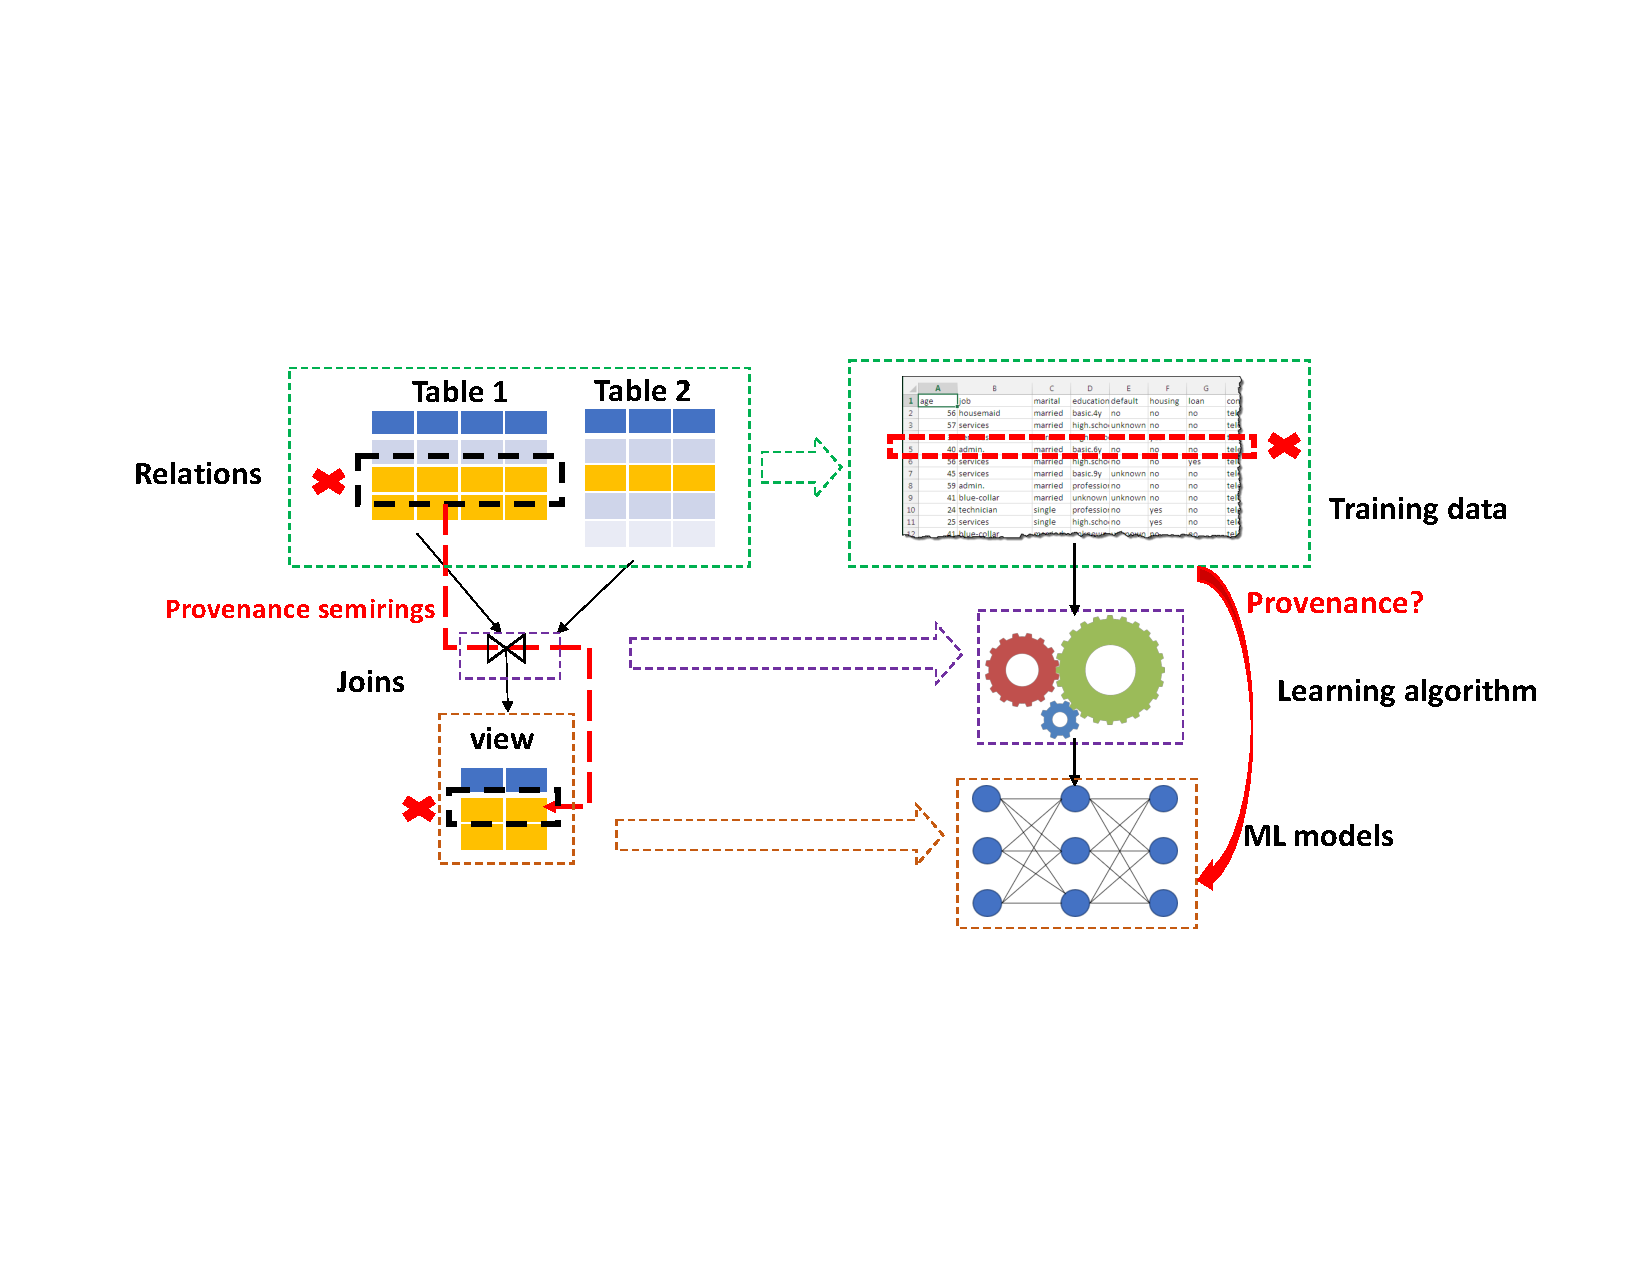
\includegraphics[width=0.75\textwidth, bb = 100pt 0pt 600pt 250pt]{figs/Updating -rev.pdf}
\caption{Parallels between materialized view maintenance 
%based on provenance semirings~\cite{GreenKT07} 
and model maintenance}
\label{fig:view-update}
\end{center}
\end{figure}

One very effective technique for materialized view maintenance is based on provenance, in particular the {\em provenance semiring} framework~\cite{GreenKT07}.  In this setting, by tracing the use of input tuples for each tuple in the view using {\em provenance polynomials}, the deletion of an input tuple can be propagated to a view tuple by seeing how and if it is used in the view tuple's provenance polynomial.

Of course, a machine learning algorithm is much more complicated than a relational algebra expression.  However, recent work has extended the provenance semiring framework to linear algebra operations~\cite{yan2016fine}, opening the door to using provenance to reason over ML algorithms based on those operations, such as {\em linear regression} and {\em logistic regression} in which non-linear operations are linearized using piecewise linear interpolation~\cite{wu2020priu}.  
In this paper, we show how provenance can be used for incrementally updating machine learning models for linear or logistic regression in our \priu\ system~\cite{wu2020priu}.  In particular we show how provenance information carried by the linear operations can be cached during the model training process and then reused for speeding up the model maintenance.
For more complex models which use non-linear operations, provenance is not yet defined. However, building on the ideas used in \priu\ of caching essential intermediate results, we therefore show how caching can be used to incrementally update more complex models (such as neural networks) in
our \deltagrad\ system~\cite{wu2020deltagrad}.

% \eat{
% In this paper, we show how provenance can be used {\em explicitly} for incrementally updating machine learning models for linear or logistic regression in our \priu\ system~\cite{wu2020priu}, as well as {\em implicitly} for more complex models (such as neural networks) in our \deltagrad\ system~\cite{wu2020deltagrad}. For the former case, the provenance information carried by the linear operations is {\em explicitly} cached during the model training process, which is then reused for speeding up the model maintenance. For the latter case, instead of leveraging explicit provenance information, which is not defined for the non-linear operations in more complex models, we determined to reuse some essential intermediate results collected in the training process, which could be regarded as an implicit way to use provenance.
% }

% By ``implicitly" we mean that certain information is cached during the model training process, and reused to speed up the model maintenance.
%\val{Unclear what "implicitly" means here and what "caching" means later in the sentence; you need to take time and use a whole sentence to explain}
%\susan{Yinjun, please look at this.  Need to make sure that the use of provenance implicitly is clear in \deltagrad\ (caching $\neq$ provenance). If it really is just caching, then we need to say that ideas from provenance-based model maintenance (e.g. caching intermediate results that can be quickly updated using provenance) inspired our use of caching in more complex models... but not that it is provenance that is being used.}\yinjun{I think it is true that caching $\neq$ provenance. I thus modify the above sentences a little bit. Not sure whether my claims above are accurate or not...}
%\susan{rewrote}

We then explore the connection of our provenance-based technique to other {\em machine unlearning} techniques (e.g.,~\cite{bourtoule2021machine}).  A major concern in machine unlearning is that the unlearned model may suffer from \emph{model inversion attacks}~\cite{fredrikson2015model}, in which the adversary is able to restore the deleted data items (a.k.a {\em private} data) from the resulting model either using just the model (a {\em black box} attack) or using auxiliary information such as the model type, model parameters, or even the remaining training samples (a {\em white box} attack).  In contrast to other machine unlearning techniques, we show that a benefit of our provenance-based technique is that it can avoid such attacks with low overhead and without loss of prediction performance.

% \eat{ We need to develop an unlearning algorithm that outputs the same distribution of models as retraining without d_u (the naive solution), which is our (strict) deterministic definition that we explore to better align with the goals of new privacy legislation; in this setting, we certainly unlearn the entirety of d_u’s contributions. If these distributions do not match, then there is necessarily some influence from d_u that has led to this difference. Settings where an unlearning algorithm only approximately matches the retraining distribution can be viewed as a (relaxed) probabilistic setting, where we unlearn most (but not all) of d_u’s contributions.}

The remainder of this paper is organized as follows:  In Section~\ref{sec: background} we give background information on provenance semirings and deletion propagation.  In Section~\ref{sec: overview} we discuss how to extend these ideas to incremental model maintenance for linear and logistic regression models in our system \priu, and for more complex models in our system \deltagrad.  We then discuss the problem of model inversion attacks in Section~\ref{sec: security}, and show how our framework can be used to guard against them.

\section{Background}
\label{sec: background}

We start by describing the provenance semiring framework in relational databases, and how provenance can be used to incrementally update views.  We then discuss how the framework has been extended to include linear algebra operations

\paragraph*{Provenance Semirings.}
%The provenance semiring framework~\cite{green2007provenance, amsterdamer2011provenance, yan2016fine} has been used for propagating deletions to views.
In the provenance semiring framework~\cite{GreenKT07}, input data to a query is annotated with
provenance tokens which are propagated through the algebraic operators performed on the data, e.g. select, project, join, union, and more recently aggregation~\cite{amsterdamer2011provenance}.
As the provenance annotations propagate, they are combined using two abstract operations.
The provenance operation $\otimes$ signifies {\em joint use} of data. For example, when tuple $t_1$,
respectively $t_2$, are annotated with provenance $p$, respectively $q$, then the tuple obtained by
joining $t_1$ and $t_2$ is annotated with provenance $p\otimes q$. The other provenance operation, $\oplus$, signifies {\em alternative use} of data. For example, when tuple $t_1$, respectively $t_2$, are annotated with provenance $p$, respectively $q$, such that $t_1$ and $t_2$ project to the same
tuple $t$, then the resulting tuple $t$ is annotated with provenance $p\oplus q$. In addition,
an abstract "zero-polynomial" $0_{prov}$ is used to annotate \emph{absent} tuples and an abstract "unit-polynomial" $1_{prov}$ is used to annotate 
"neutral" data whose provenance is ignored (it's of no interest in a specific analysis). If $P$ is the mathematical space of provenance annotations, standard equivalences of positive relational algebra
imply that $(P,\oplus,\otimes,0_{prov},1_{prov})$ is a \emph{commutative semiring}~\cite{GreenKT07}. It follows that
the expressions obtained as provenance is propagated through a query can be put in standard polynomial form, where the indeterminates (the variables) are provenance tokens that annotate the tuples in the data given as input to the query. Therefore, in the semiring framework provenance is captured by \emph{provenance polynomials}.



\example{As an example, suppose we have two tables, $R$ and $S$, whose tuples are annotated with provenance tokens $p$, $q$, and $r$, as shown in Figure~\ref{fig:prov-propag}.  In the same figure 
we show the provenance polynomials in indeterminates $p,q,r$ that are produced by provenance propagation in the outputs of queries $R\bowtie_B S,~~\Pi_{A, C} R$, and $\Pi_{A, D} (R \times S)$.
As is customary in algebra, we omit the multiplication-like symbol $\otimes$ when we write polynomials in commutative indeterminates.
%\val{YINJUN PLEASE FIX THE DISPLAY IN FIGURE 2}\yinjun{Done, can you take a look?}
}


\begin{figure}
\begin{center}
%  \begin{table}
  \centering\small
  \begin{tabular}{|c|c|c||c}
  \multicolumn{4}{l}{$R$}\\
  A & B & C \\ \cline{1-3}
  a1 & b1 & c1& $p$\\
   a1 & b2 & c1& $q$\\
 \end{tabular}
  \hspace{0.3in} 
  \centering\small
  \begin{tabular}{|c|c|c||c}
  \multicolumn{4}{l}{$S$}\\
  D & B & E \\ \cline{1-3}
  d1 & b1 & e1 & $r$\\
  \end{tabular}
  \\
 %  \hspace{0.3in}
  \centering\small
  \begin{tabular}{|c|c|c|c|c||c}
  \multicolumn{6}{l}
  {$R \bowtie_B S$}\\
  A & B & C & D & E\\ \cline{1-5}
  a1 & b1 & c1& d1& e1 & $pr$\\
  \end{tabular}
   \hspace{0.3in} 
  \centering\small
  \begin{tabular}{|c|c||c}
  \multicolumn{3}{l}
  {$\Pi_{A, C} R$}\\
  A & C \\ \cline{1-2}
  a1 & c1 & $p\oplus q$\\
  \end{tabular}
  \hspace{0.3in} 
  \centering\small
  \begin{tabular}{|c|c||c}
  \multicolumn{3}{l}
  {$\Pi_{A, D} (R \times S)$}\\
  A & D \\ \cline{1-2}
  a1 & d1 & $pr\oplus qr$.\\
  \end{tabular}
%\end{table}
\end{center}
\caption{Provenance propagation}
\label{fig:prov-propag}
\end{figure}

\paragraph*{Deletion Propagation.}
One of the benefits of the semiring framework is that deletions of tuples in the input tuples propagate straightforwardly to deletions (or modifications of provenance) of output tuples  
by partially evaluating provenance polynomials using familiar algebraic rules.

When an input tuple is deleted, the effect on the output can be efficiently calculated by setting its token to $0_{prov}$ in the output's provenance polynomials, signifying absence.  For example, if the first tuple in $R$, (a1, b1, c1) with provenance token $p$, were deleted, then the provenance of the (only) tuple in $R \bowtie_B S$ would become $0_{prov}\otimes r= \; 0_{prov}$, indicating that it no longer appears -- intuitively, both tuples are needed for that tuple to be present.  On the other hand, the tuple in $\Pi_{A, C}R$ would still appear but with a different provenance $0_{prov}\oplus q= \; q$ -- intuitively, at least one of $p$ and $q$ is needed for the result to be present. Similarly, deleting the first tuple in $R$ will still leave the tuple (a1,d1) in the output of $\Pi_{A, D} (R \times S)$, but its provenance would become $(0_{prov}\otimes r) \oplus (q\otimes r)\;=\; 0_{prov}\oplus (q\otimes r) \;=\; qr$.


\paragraph*{Extension to Linear Algebra Operations}
Recently, the semiring framework has been extended to include basic linear algebra operations: matrix
addition and multiplication~\cite{yan2016fine}. In this extension, the provenance polynomials play the role of abstract scalars and an abstract version of multiplication with scalars plays the role of annotating matrices (in particular, vectors) with provenance. Matrices form a non-commutative, many-sorted ring. The structure obtained by combining the ring of matrices with multiplication by scalars from the semiring of provenance polynomials is a \emph{semialgebra}~\cite{yan2016fine}.
This framework is flexible enough that for input matrices we can annotate both rows (samples)
and columns (features) with arbitrary provenance tokens.

As an example, suppose that $p$,$q$,$r$,$s$ are provenance tokens that annotate four different samples in a training dataset. We denote the multiplication with scalars (i.e., the annotation with provenance polynomias) by the abstract operation $*$. Using the work in~\cite{yan2016fine}, our methods will show that vectors of interest (such as the vector
of model parameters) can be expressed with provenance annotated expressions such as:
\begin{small}
\begin{align}\label{eq: w}
     \w = (p^2q*\u) + (qr^4*\v) + (ps*\z)
\end{align}
\end{small}

Here, $\u$,$\v$,$\z$ are numerical vectors signifying contributions
to the answer $\w$ and they are annotated with the provenance polynomials $p^2q$, $qr^4$, $ps$.

Now suppose the sample (input row) annotated with
$r$ is deleted while those annotated $p$,$q$,and $s$ are retained but we decide not to track them anymore. As we did in the paragraph on deletion
propagation, we can express the updated value of $\w$ under this deletion by setting $r$ to  $0_{prov}$ which signifies absence, 
and $p$,$q$,$s$ to $1_{prov}$, which signifies “neutral” presence in Equation~(\ref{eq: w}). Again, the resulting expressions
can be simplified using familiar algebraic manipulations. As expected,
%The algebraic properties of provenance polynomials and 
%of their annotation of matrices/vectors ensure what one would expect, e.g, 
$0_{prov}\otimes r^4$ = $0_{prov}$ as well as
$0_{prov}*\v = \mathbf{0}$ (the all-zero vector). Moreover,  $1_{prov}\otimes 1_{prov} = 1_{prov}$
and $1_{prov}*\z = \; \z$. It follows
that under this deletion $\w = \; \u + \z$.



% %!TEX root = ../main.tex
\section{Related Works}
\label{sec:related}

\stitle{Retrieval Augmented Generation Question Answering.}
%
Large languaga models sometimes generate factually incorrect or misleading information, often due to a lack of real-time knowledge or limited access to external facts beyond their training data.
RAG-based Question Answering addresses this by integrating external knowledge retrieval into the generation process. By retrieving relevant document chunks through semantic search, RAG ensures that the model’s responses are grounded in accurate, real-world information, effectively reducing the likelihood of hallucinations.
Early approaches focused on jointly training the retriever and generator, ensuring that the retrieved content aligned with the generation model’s intent to provide more accurate answers~\cite{izacard2023atlas}. With the success of in-context learning, more recent work has treated the retriever as a separate module, directly providing retrieved information to the model via prompts~\cite{wang2023knowledgptenhancinglargelanguage}.
As retrieval technologies have advanced, RAG-based systems now support multimodal retrieval, enabling answers that draw from diverse data sources~\cite{chen2021open, chen-etal-2022-murag, luo-etal-2023-unifying}. 
%For example, OTT-QA~\cite{chen2021open}  retrieves both tables and text, MuRAG~\cite{chen-etal-2022-murag} integrates text and images, and MMQA~\cite{luo-etal-2023-unifying} combines text, tables, and images to handle complex queries.
% \yang{It's hard for us to compare Symphony with existing systems.}


\stitle{Trustworthiness of Large Language Models.}
%
The trustworthiness of LLMs is essential for their effective deployment in real-world applications. To assess LLM trustworthiness, researchers have proposed various approaches. For example, TrustLLM~\cite{huang2024trustllmtrustworthinesslargelanguage} provides a comprehensive framework for evaluating LLMs across different trust dimensions.
However, evaluating LLM trustworthiness remains challenging, with gaps in holistic assessment approaches. Some studies suggest that self-evaluation, where LLMs assess their confidence in the generated outputs, can help improve selective generation and mitigate inaccuracies~\cite{Ren2023SelfEvaluationIS}. Additionally, understanding the internal mechanisms of LLMs, such as the use of local intrinsic dimension (LID) for predicting truthfulness, has been proposed as a way to measure model reliability~\cite{Yin2024CharacterizingTI}.
In our work, we aim to improve the trustworthiness of LLMs through post-verification, ensuring that generated outputs are validated against reliable sources after generation to minimize inaccuracies and enhance their overall reliability.
 
% %!TEX root=../2022_IEEE_DEB_Vizier.tex

% %%%%%%%%%%%%%%%%%%%%%%%%%%%%%%%%%%%%%%%%
% \begin{figure}[t]
%   \centering
%   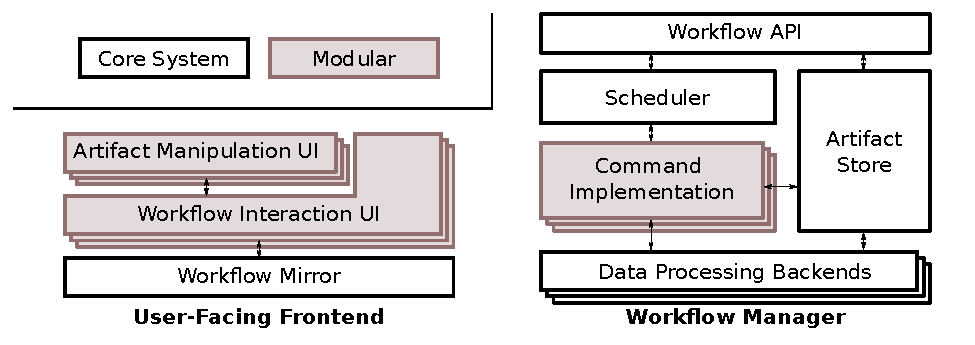
\includegraphics[width=0.7\textwidth]{graphics/systemarch}\\[-5mm]
%   \caption{Vizier's architecture, comprised of a user-facing frontend component and a backend component.}\label{fig:vizier-architecture}
% \end{figure}
% %%%%%%%%%%%%%%%%%%%%%%%%%%%%%%%%%%%%%%%%

%%%%%%%%%%%%%%%%%%%%%%%%%%%%%%%%%%%%%%%%%%%%%%%%%%%%%%%%%%%%%%%%%%%%%%%%%%%%%%%%
\pagebreak[4]
\subsection{Solution Overview}
\label{sec:solution-overview}

%%%%%%%%%%%%%%%%%%%%%%%%%%%%%%%%%%%%%%%%
\begin{wrapfigure}[12]{r}[0pt]{12cm}
  \centering
  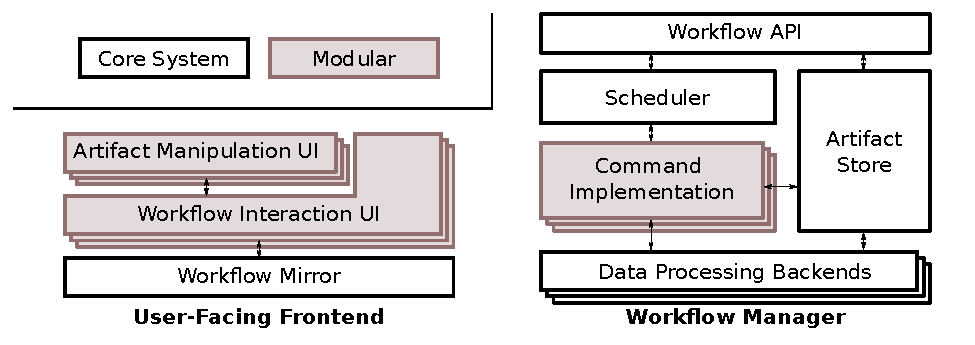
\includegraphics[width=0.7\textwidth]{graphics/systemarch}\\[-5mm]
  \caption{Vizier's architecture, comprised of a user-facing frontend component and a backend component.}\label{fig:vizier-architecture}
\end{wrapfigure}
%%%%%%%%%%%%%%%%%%%%%%%%%%%%%%%%%%%%%%%%
An overview of Vizier's architecture is shown in \Cref{fig:vizier-architecture}.
Addressing requirement \textbf{W1}, the central abstraction in Vizier is a workflow: a linear sequence of steps. % taken by the user in pursuit of a specific objective.
Unlike classical workflow systems, Vizier does not require users to explicitly declare information flow between steps.
Rather Vizier borrows the model employed in popular computational notebooks like Jupyter, where inter-cell communication occurs through a global state (artifacts) passed sequentially through steps.
Following notebook conventions, we refer to these steps as \emph{cells}, and the global state as a \emph{scope}, a map from artifact name to the version of the artifact valid at this point in the workflow. Vizier stores artifacts in common formats through a versioned \textbf{Artifact Store} (\Cref{sec:data-artifacts}), addressing requirement \textbf{A2}.
In \Cref{sec:vizier-workflows}, we formalize Vizier's workflow model, and show how we satisfy requirement \textbf{W3} by instrumenting how each cell interacts with the scope, allowing us to determine what artifact versions are valid.

Vizier's workflow semantics, paired with the versioned artifact store and workflow versioning (\Cref{sec:vizier-history}) addresses requirement \textbf{W2}. % as notebooks have a natural concept of logical order (the order of cells in the notebook) that can be adjusted over time.
% Adding workflow versioning  is sufficient to fully address the requirement.
In contrast, classical notebooks like Jupyter or Zeppelin rely on the global state of an interpreter for inter-cell communication.
Reverting this state to an earlier revision is challenging~\cite{zelnicki:2017:nodebook}, limiting their ability to satisfy requirement \textbf{W3}.
Vizier instead relies on its versioning system, allowing its \textbf{Scheduler} to automatically detect and re-evaluate stale cells (\Cref{sec:vizier-scheduler}).
To address requirement \textbf{A3}, we designed a light-weight uncertain data model that is implemented in Vizier in the form of \textit{caveats}, annotations on data that indicate uncertain values and rows  (\Cref{sec:data-docum-error}).

Addressing requirement \textbf{A1} requires modularity in both Vizier's front- and back-end components.
First, the user's interactions with a workflow and artifacts, whether through a scripting language, graphical interaction, or any other modality, need to be captured for replay (simultaneously addressing requirement \textbf{A4}). In Vizier this is achieved by requiring that every update to an artifact made through a particular modality has to be reflected as an operation in the workflow, i.e., a data update is translated into a workflow update.
Vizier manages a collection of \textbf{Command Implementations} that implement the logic behind these artifact transformations (\Cref{sec:multimodality}).
To streamline the implementation of commands, Vizier's data formats and transformations are built over standard \textbf{Data Processing Backends} like Apache Spark.
% For example, Vizier supports fine-grained provenance over datasets by encoding them as Spark data frames.

The frontend is implemented over a \textbf{Workflow Mirror} that uses websockets to reflect a live view of the workflow the user is editing.
Vizier automatically derives a default \textbf{Artifact Manipulation User Interface} for its notebook interface from each command's parameter schemas. This interface suffices for many templated commands, but the frontend can be further extended to provide a more customized experience, for example for Spreadsheet-style direct manipulation of data (\Cref{sec:spreadsheets}).
As illustrated in \Cref{fig:screenshot}, the frontend displays three \textbf{Workflow Interaction User Interfaces} by default: (i) A direct display of the workflow as a notebook, (ii) a table of contents summary of the notebook, including highlighting from documentation, and (iii) a list of artifacts derived by the notebook.
Several of these components, including the notebook and the artifact list provide access to direct manipulation interfaces.
Additional views currently implemented in Vizier include: (iv) A caveat view (\Cref{sec:data-docum-error}) that shows and tracks potential errors in the workflow and data, (v) a history view that shows the evolution of the workflow over time, and (vi) a data provenance subway diagram view.

%%%%%%%%%%%%%%%%%%%%%%%%%%%%%%%%%%%%%%%%%%%%%%%%%%%%%%%%%%%%%%%%%%%%%%%%%%%%%%%%
\begin{figure}
  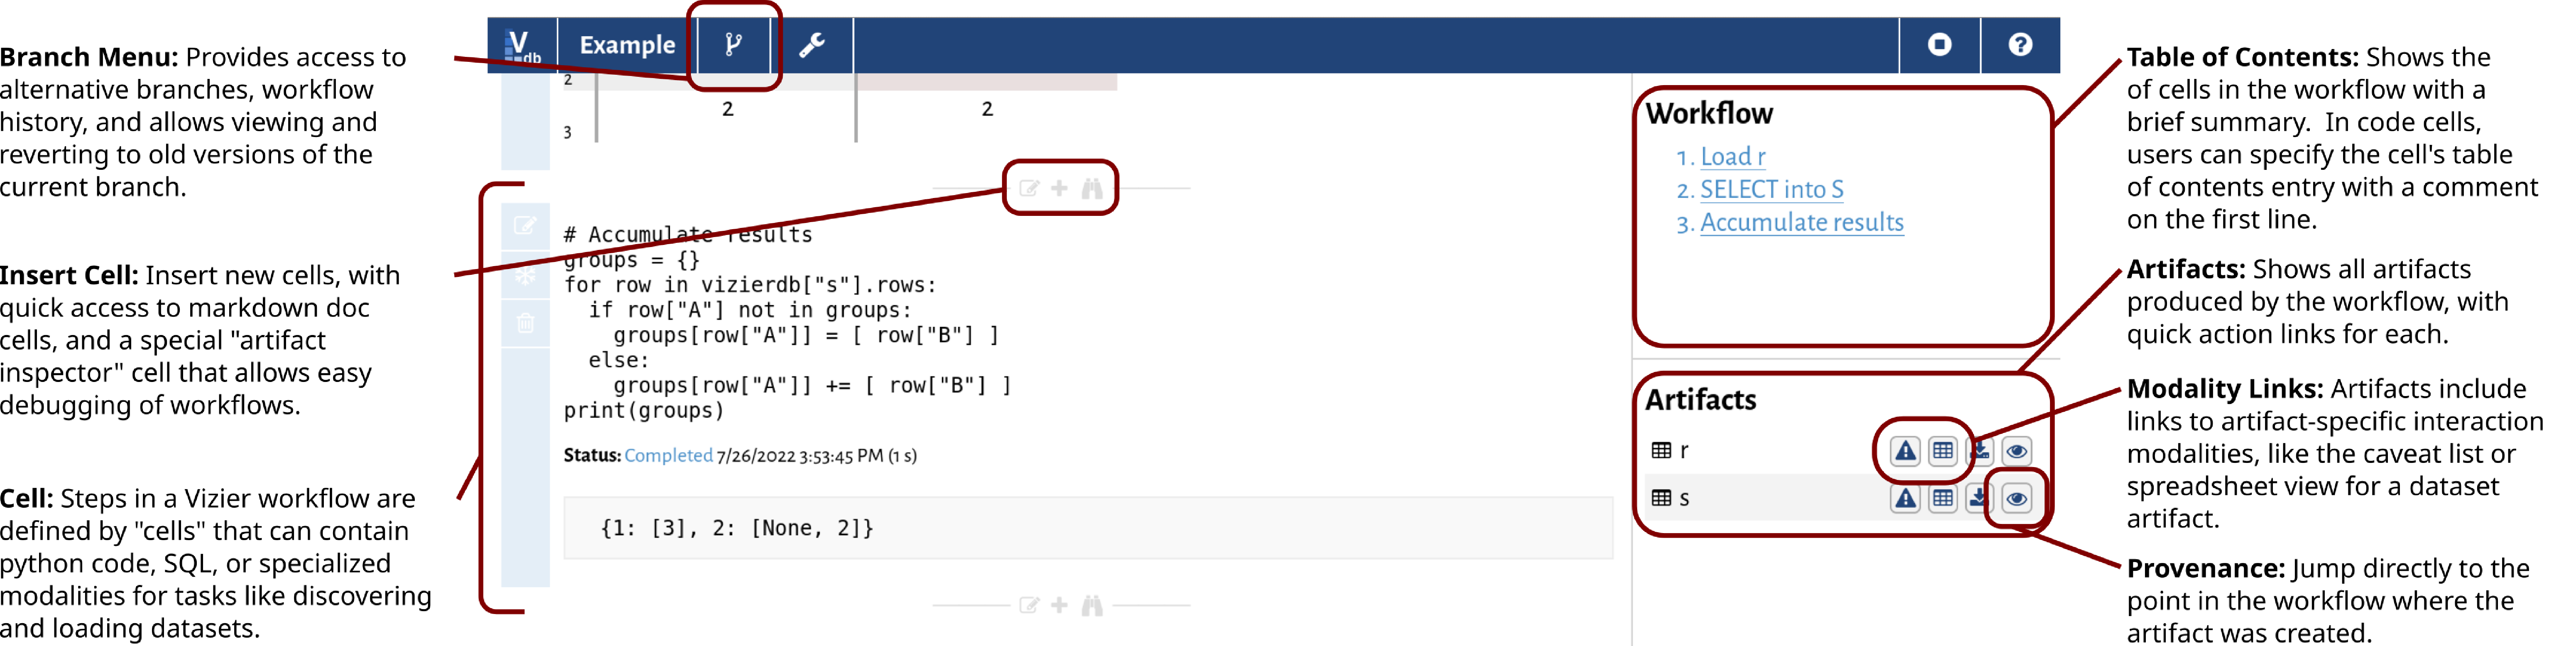
\includegraphics[width=\textwidth]{graphics/screenshot.pdf} 
  \caption{The Vizier User Interface}
  \label{fig:screenshot}
\end{figure}
%%%%%%%%%%%%%%%%%%%%%%%%%%%%%%%%%%%%%%%%%%%%%%%%%%%%%%%%%%%%%%%%%%%%%%%%%%%%%%%%

%%% Local Variables:
%%% mode: latex
%%% TeX-master: "../2022_IEEE_DEB_Vizier"
%%% End:

\section{Overview of \priu\ and \deltagrad}
\label{sec: overview}
%sgd and math preliminary

We start with preliminaries on Stochastic Gradient Descent (SGD) before showing the explicit use of provenance in \priu\ and the implicit use of provenance in \deltagrad\ for incrementally updating machine learning models in \deltagrad.

\subsection{Preliminaries on SGD}
By assuming that SGD is used for model training, \priu\ and \deltagrad\ can incrementally update the ``gradients'' at each SGD step. Suppose the training dataset is $D_{\text{train}}=\{(\x_i, \y_i)\}_{i=1}^n$ and model parameter is $\w$, at the step $t$ of SGD 
% \val{I suggest step $t$ of SGD instead}
% \yinjun{Yes, I reword it}, 
$\w$ is computed by evaluating the gradients on a randomly sampled mini-batch of the training dataset, i.e.:
\begin{small}
\begin{align}\label{eq: sgd}
    % \w_{t+1} = \w_{t} - \eta_t\cdot\underbrace{\frac{1}{|\miniB_{t}|}\sum_{i \in \miniB_{t}} \nabla F\left(\w_{t}; (\x_i,\y_i)\right)}_{\text{$\text{Grad}(\w_t; \miniB_t)$}},
     \w_{t+1} = \w_{t} - \eta_t \cdot \text{Grad}(\w_t; \miniB_t),
    %  \eta_t\cdot\underbrace{\frac{1}{|\miniB_{t}|}\sum_{i \in \miniB_{t}} \nabla F\left(\w_{t}; (\x_i,\y_i)\right)}_{\text{$\text{Grad}(\w_t; \miniB_t)$}},
\end{align}
\end{small}

\noindent
where $\text{Grad}(\w_t; \miniB_t)$ represents the gradient evaluated on a mini-batch $\miniB_t$. 

%sgd after removal
Suppose a subset of training samples, $R$, is removed from the training dataset.  Then to compute the updated model parameter, Equation \eqref{eq: sgd} is modified as:
\begin{small}
\begin{align}\label{eq: sgd_update0}
    % \uw_{t+1} = \uw_{t} - \eta_t\cdot\underbrace{\frac{1}{|\miniB_{t} - R|}\sum\nolimits_{i \in \miniB_{t} - R} \nabla F\left(\uw_{t}; (\x_i,\y_i)\right)}_{\text{$\text{Grad}(\w_t; \miniB_t - R)$}},
    \uw_{t+1} = \uw_{t} - \eta_t\cdot \text{Grad}(\w_t; \miniB_t - R)
    % \underbrace{\frac{1}{|\miniB_{t} - R|}\sum\nolimits_{i \in \miniB_{t} - R} \nabla F\left(\uw_{t}; (\x_i,\y_i)\right)}_{\text{$\text{Grad}(\w_t; \miniB_t - R)$}},
\end{align}
\end{small}
\noindent
where $\uw$ represents the updated model parameter and $\miniB_{t} - R$ represents the remaining samples in $\miniB_t$ after the removal of $R$.

Note that both $\text{Grad}(\w_t; \miniB_t)$ in Equation \eqref{eq: sgd} and $\text{Grad}(\w_t; \miniB_t - R)$ in Equation \eqref{eq: sgd_update0} can be regarded as the integration of two components: the model parameter $\w_t$ (or $\uw_t$) and the data part (the sample $(\x_i, \y_i)$). For example, for linear regression models, the loss function $F\left(\w_t; (\x_i, \y_i)\right)$ using L2 regularization is $$F\left(\w_{t}, (\x_i,\y_i)\right) = (y_i - \x_i^\top\w)^2 + \frac{\lambda}{2}\|\w_t\|^2,$$
Using this, $\text{Grad}(\w_t; \miniB_t)$ and $\text{Grad}(\w_t; \miniB_t - R)$ can be rewritten as:
\begin{small}
\begin{align}\label{eq: linear_regression_sgd}
    \begin{split}
        \text{Grad}(\w_t; \miniB_t) = (\lambda\textbf{I} + \frac{2}{|\miniB_t|}\sum\nolimits_{i \in \miniB_t} \x_i\x_i^\top)\w_t  - \frac{2}{|\miniB_t|}\sum\nolimits_{i \in \miniB_t}\x_i \y_i,
    \end{split}\\
    \begin{split}\label{eq: linear_regression_sgd_update0}
    \text{Grad}(\w_t; \miniB_t-R) = (\lambda\textbf{I} + \frac{2}{|\miniB_t - R|}\sum\nolimits_{i \in \miniB_t - R} \x_i\x_i^\top)\uw_t  - \frac{2}{|\miniB_t-R|}\sum\nolimits_{i \in \miniB_t-R}\x_i \y_i
\end{split}
\end{align}
\end{small}

The data part in $\text{Grad}(\w_t; \miniB_t)$ (Equation \eqref{eq: linear_regression_sgd}) consists of two terms:
\begin{small}
\begin{align*}
D_1(\miniB_t) = \sum\nolimits_{i \in \miniB_t} \x_i\x_i^\top, \; D_2(\miniB_t) = \sum\nolimits_{i \in \miniB_t}\x_i \y_i.    
\end{align*}
\end{small}

Similarly, the data part in $\text{Grad}(\w_t; \miniB_t-R)$ (Equation \eqref{eq: linear_regression_sgd_update0} can be expressed as: 
\begin{small}
\begin{align*}
D_1(\miniB_t - R) = \sum\nolimits_{i \in \miniB_t - R} \x_i\x_i^\top, \; D_2(\miniB_t - R) = \sum\nolimits_{i \in \miniB_t-R}\x_i \y_i.    
\end{align*}
\end{small}


\subsection{\priu}
As described above, by decomposing the gradient formulas $\text{Grad}(\w_t; \miniB_t)$ or $\text{Grad}(\w_t; \miniB_t - R)$ into a data part and a model parameter part, we can \emph{capture the provenance of the data part to track how the changes of the data part lead to the updates of the model parameters at each SGD iteration}. 
% For the above example, we can employ the provenance of $D_1(\miniB_t)$ and $D_2(\miniB_t)$ to achieve effective update on 
% It is worth noting that the only differences between the data parts in $\text{Grad}(\w_t; \miniB_t)$ and $\text{Grad}(\w_t; \miniB_t - R)$ are the removed sample part. This thus motivates us to capture the provenance for the terms, $D_1(\miniB_t)$ and $D_2(\miniB_t)$ in $\text{Grad}(\w_t; \miniB_t)$ such that this provenance can be employed to incrementally evaluate $\text{Grad}(\w_t; \miniB_t - R)$ after the removal of $R$.

Specifically, for the above example, suppose each training sample $(\x_i, \y_i)$ is given a unique provenance token, $p_i$.  Then we can generate the following provenance-aware formula for $D_1(\miniB_t)$ and $D_2(\miniB_t)$:
\begin{small}
\begin{align*}
    &\text{Prov}(D_1(\miniB_t)) = \sum\nolimits_{i \in \miniB_t} p_i^2*\x_i\x_i^\top, \text{ Prov}(D_2(\miniB_t)) =  \sum\nolimits_{i \in \miniB_t}p_i^2*\x_i \y_i
\end{align*}
\end{small}

To obtain the values of $D_1(\miniB_t - R)$ and $D_2(\miniB_t - R)$, we can set the provenance token $p_i $ to $0_{{prov}}$ for each $i\in R$ to zero out the removed training samples, and set the other provenance tokens to $1_{{prov}}$, i.e.:
\begin{small}
\begin{align*}
    & D_1(\miniB_t - R) = \sum\nolimits_{i \in \miniB_t - R} \x_i\x_i^\top = [\sum\nolimits_{i \in \miniB_t - R} p_i^2*\x_i\x_i^\top]_{p_i = 1_{{prov}}} + [\sum\nolimits_{i \in \miniB_t \bigcap R} p_i^2*\x_i\x_i^\top]_{p_i = 0_{{prov}}}\\
    % = D_1(\miniB_t) - \sum\nolimits_{i \in \miniB_t \bigcap R} \x_i\x_i^\top\\
    & D_2(\miniB_t - R) = \sum\nolimits_{i \in \miniB_t - R}\x_i \y_i = [\sum\nolimits_{i \in \miniB_t - R} p_i^2*\x_i\y_i]_{p_i = 1_{{prov}}} + [\sum\nolimits_{i \in \miniB_t \bigcap R} p_i^2*\x_i\y_i]_{p_i = 0_{{prov}}}
\end{align*}
\end{small}

This can be implemented by reusing the cached terms, $D_1(\miniB_t)$ and $D_2(\miniB_t)$ and subtracting the terms corresponding to the removed samples in $R$, i.e.:
\begin{small}
\begin{align*}
    & D_1(\miniB_t - R) = \sum\nolimits_{i \in \miniB_t - R} \x_i\x_i^\top 
    % = [\sum\nolimits_{i \in \miniB_t - R} p_i^2*\x_i\x_i^\top]_{p_i = 1_{{prov}}} + [\sum\nolimits_{i \in \miniB_t \bigcap R} p_i^2*\x_i\x_i^\top]_{p_i = 0_{{prov}}}\\
    = D_1(\miniB_t) - \sum\nolimits_{i \in \miniB_t \bigcap R} \x_i\x_i^\top\\
    & D_2(\miniB_t - R) = \sum\nolimits_{i \in \miniB_t - R}\x_i \y_i = D_2(\miniB_t) - \sum\nolimits_{i \in \miniB_t \bigcap R} \x_i\y_i
\end{align*}
\end{small}
\noindent
This is considerably more efficient than recomputing $D_1(\miniB_t - R)$ and $D_2(\miniB_t - R)$ from scratch  if the size of $R$ is much smaller than the total number of training samples.




% to track which part of samples are removed or not such that 

%intuition of the two methods


%intro to priu

% \eat{So far, we have discussed how to capture and reuse the provenance of the data part in the SGD formulas where the data part and the model parameters are {\em linearly combined} such that $\text{Grad}(\w_t; \miniB_t)$ can be effectively updated to $\text{Grad}(\w_t; \miniB_t - R)$ after the removal of the training sample set, $R$. However, it is worth noting that in general cases, the term, $\text{Grad}(\w_t; \miniB_t)$ can be more complicated, in which the data part and the model parameters can be integrated in an arbitrary way, thus complicating the way to employ the provenance. }
So far, we have discussed how to efficiently update $\text{Grad}(\w_t; \miniB_t)$ to $\text{Grad}(\w_t; \miniB_t - R)$ after the removal of a training sample set 
% \eat{by capturing and reusing the provenance of the data part}
for SGD formulas where the data part and the model parameters are {\em linearly combined}. 
However, in general cases the data part and the model parameters in $\text{Grad}(\w_t; \miniB_t)$ can be integrated in an arbitrary way, making it difficult to use provenance.
% In \priu, we started from a simple case, i.e., how to follow the above intuition to incrementally update linear models, e.g., linear regression and 
For example, for {\em logistic regression with L2 regularization} the loss function, $F(\cdot)$, and $\text{Grad}(\w_t; \miniB_t)$, can be instantiated as:

\begin{small}
% \begin{align}\label{eq: linear_regression_grad}
% \begin{split}
%     \text{Linear regression: } & F\left(\w_{t}, (\x_i,\y_i)\right) = (y_i - \x_i^\top\w)^2 + \frac{\lambda}{2}\|\w_t\|^2,\\
%     &\text{$\text{Grad}(\w_t; \miniB_t)$} 
%     % = \lambda\w_{t} + 2\frac{1}{|\miniB_t|}\sum\nolimits_{i \in \miniB_t} \x_i(\x_i^T\w_t - \y_i)
%     % = \lambda\w_{t} + \frac{2}{|\miniB_t|}\sum\nolimits_{i \in \miniB_t} \x_i\x_i^T\w_t  - \frac{2}{|\miniB_t|}\sum\nolimits_{i \in \miniB_t}\x_i \y_i
%     = (\lambda\textbf{I} + \frac{2}{|\miniB_t|}\sum\nolimits_{i \in \miniB_t} \x_i\x_i^T)\w_t  - \frac{2}{|\miniB_t|}\sum\nolimits_{i \in \miniB_t}\x_i \y_i
% \end{split}
% \end{align}
% \eat{
% \begin{align}\label{eq: logistic_regression_grad}
% \begin{split}
%     & F\left(\w_{t}, (\x_i,\y_i)\right) = \ln (1+\exp\{-\y_i\w^\top_t\x_i\}) + \frac{\lambda}{2}\|\w_t\|^2, \text{$\text{Grad}(\w_t; \miniB_t)$} = \lambda\w_t -  \frac{1}{|\miniB_t|}\sum\nolimits_{i \in \miniB_{t}} \y_i\x_i (1-\frac{1}{1+\exp\{-y_i\w_{t}^\top\x_i\}})
% \end{split}
% \end{align}
% % \end{small}
% }

\begin{align}
    & F\left(\w_{t}, (\x_i,\y_i)\right) = \ln (1+\exp\{-\y_i\w^\top_t\x_i\}) + \frac{\lambda}{2}\|\w_t\|^2 \\
    \label{eq: logistic_regression_grad}
    & \text{Grad}(\w_t; \miniB_t) = \lambda\w_t -  \frac{1}{|\miniB_t|}\sum\nolimits_{i \in \miniB_{t}} \y_i\x_i (1-\frac{1}{1+\exp\{-y_i\w_{t}^\top\x_i\}})
\end{align}
\end{small}


% in which we assume that these models are regularized by $\frac{\lambda}{2}\|\w_t\|^2$ with $\lambda$ as the hyper-parameter. 

%intuition of priu for linear regression
% Note that in Equation \eqref{eq: linear_regression_grad}, the model parameter, $\w_t$, and the data part (i.e. the terms composed of $\x_i$ or $\y_i$) are linearly combined. This indicates that by simply caching the data part (e.g., $\frac{2}{|\miniB_t|}\sum\nolimits_{i \in \miniB_t} \x_i\x_i^T$ and $\frac{2}{|\miniB_t|}\sum\nolimits_{i \in \miniB_t}\x_i \y_i$) and reusing it with a different model parameter, e.g., $\uw_t$, the updated $\text{Grad}(\w_t; \miniB_t)$, i.e., $\text{Grad}(\w_t; \miniB_t - R)$, could be effectively evaluated without recomputing the data part from scratch.

%how to apply the intuition above for logistic regression
\noindent
in which the model parameter $\w_t$ and the data part are combined with non-linear operations 
(i.e., $\exp$ and division).
% \eat{
% Therefore, as the first step to capture the provenance for the data part, it is essential to conduct further transformations on $\text{Grad}(\w_t; \miniB_t)$ in Equation \eqref{eq: logistic_regression_grad} to disentangle the data part from its combination with the model parameters. 
% % This can thus facilitate capturing the provenance in the data part. 
% }
To be able to use provenance for rapid updates, we therefore linearize the non-linear operations in Equation \eqref{eq: logistic_regression_grad} using {\em piecewise linear interpolation}, which leads to the following ``Linearized $\text{Grad}(\w_t; \miniB_t)$'':
\begin{small}
\begin{align}\label{eq: linearized_grad_1}
    \text{Linearized $\text{Grad}(\w_t; \miniB_t)$} = \lambda\w_t -  \frac{1}{|\miniB_t|}(\sum\nolimits_{i\in \miniB_{t}}a_{i, t}\x_i\x_i^\top\w_{t} + \sum\nolimits_{i\in \miniB_t} b_{i, t}\y_i\x_i)
\end{align}
\end{small}
% is not applicable for the logistic regression model in a straightforward way. This leads to the linearization on the gradient formula

% The formula above is thus very similar to the $\text{Grad}(\w_t; \miniB_t)$ in Equation \eqref{eq: linear_regression_grad} except its additional coefficients, $a_{i,t}$ and $b_{i,t}$. 
\noindent
in which the two coefficients, $a_{i,t}$ and $b_{i,t}$, are generated after piece-wise linear interpolation is applied.
% and are associated with the subscript $i$ and $t$ due to their implicit dependence on the model parameter $\w_t$ and the sample $(\x_i, \y_i)$. 
As a consequence, Equation \eqref{eq: linearized_grad_1} shares a similar form with Equation \eqref{eq: linear_regression_sgd}, hence
%similar to the way to incrementally update the linear regression models, 
data provenance can also be used in Equation \eqref{eq: linearized_grad_1} for incrementally updating logistic regression models. Note that due to the linearization operations, the incrementally updated model parameters may not be the same as the ones retrained from scratch. However, we can prove that the difference between the two model parameters (quantified by L2 norm) is very small (see detailed analysis in \cite{wu2020priu}).
% are still very close. 
% \val{Percentage error is what?}\yinjun{reworded it}

% \eat{
% the ``data part'', i.e. $\sum\nolimits_{i\in \miniB_{t}}a_{i, t}\x_i\x_i^\top$ and $\sum\nolimits_{i\in \miniB_t} b_{i, t}\y_i\x_i$, and the model parameter are linearly combined, which is thus similar to Equation \eqref{eq: linear_regression_sgd}.  
% % Equation \eqref{eq: linearized_grad_1} becomes a linear expression of the model parameter $\w_t$ and . 
% By denoting $D^{\text{Logistic}}_1(\miniB_{t}) = \sum\nolimits_{i\in \miniB_{t}}a_{i, t}\x_i\x_i^\top$ and $D^{\text{Logistic}}_2(\miniB_t) = \sum\nolimits_{i\in \miniB_t} b_{i, t}\y_i\x_i$, we can then capture the provenance for those two expressions as follows:
% \begin{align*}
%     % \text{Prov}(\sum\nolimits_{i\in \miniB_{t}}a_{i, t}\x_i\x_i^\top) = 
%     \text{Prov}(D^{\text{Logistic}}_1(\miniB_t)) = \sum\nolimits_{i \in \miniB_t} p_i^2*a_{i,t}\x_i\x_i^\top, \text{Prov}(D^{\text{Logistic}}_2(\miniB_t)) =  \sum\nolimits_{i \in \miniB_t}p_i^2*b_{i,t}\x_i \y_i
% \end{align*}


% Then after the removal of the sample set $R$, the above provenance formula can then aid the effective update on ``Linearized $\text{Grad}(\w_t; \miniB_t)$'' with an updated model parameter, $\uw_t$ (i.e., ``Linearized $\text{Grad}(\w_t; \miniB_t - R)$''):
% \begin{small}
% \begin{align}\label{eq: linearized_grad_2}
% \begin{split}
%     &\text{Linearized $\text{Grad}(\w_t; \miniB_t - R)$} 
%     % &= \lambda\uw_t -  \frac{1}{|\miniB_t - R|}(\sum\nolimits_{i\in \miniB_{t} - R}a_{i, t}\x_i\x_i^\top\uw_{t} + \sum\nolimits_{i\in \miniB_t - R} b_{i, t}\y_i\x_i)\\
%     = \lambda\uw_t -  \frac{1}{|\miniB_t - R|}(D^{\text{Logistic}}_1(\miniB_{t}-R)\uw_{t} + D^{\text{Logistic}}_2(\miniB_{t}-R)),\\
%     & \text{where } D^{\text{Logistic}}_1(\miniB_t - R) = \sum\nolimits_{i \in \miniB_t - R} a_{i,t}\x_i\x_i^\top 
%     % = [\sum\nolimits_{i \in \miniB_t - R} p_i^2*\x_i\x_i^\top]_{p_i = 1_{{prov}}} + [\sum\nolimits_{i \in \miniB_t \bigcap R} p_i^2*\x_i\x_i^\top]_{p_i = 0_{{prov}}}\\
%     =[\sum\nolimits_{i \in \miniB_t - R} p_i^2*a_{i,t}\x_i\x_i^\top]_{p_i = 1_{{prov}}} + [\sum\nolimits_{i \in \miniB_t \bigcap R} p_i^2*a_{i,t}\x_i\x_i^\top]_{p_i = 0_{{prov}}}\\
%     % = D^{\text{Logistic}}_1(\miniB_t) - \sum\nolimits\nolimits_{i \in \miniB_t \bigcap R} \x_i\x_i^\top\\
%     & D^{\text{Logistic}}_2(\miniB_t - R) = \sum\nolimits_{i \in \miniB_t - R}b_{i,t}\x_i \y_i 
%     % = D^{\text{Logistic}}_2(\miniB_t) - \sum\nolimits_{i \in \miniB_t \bigcap R} \x_i\y_i
%     =[\sum\nolimits_{i \in \miniB_t - R} p_i^2*b_{i,t}\x_i\y_i]_{p_i = 1_{{prov}}} + [\sum\nolimits_{i \in \miniB_t \bigcap R} p_i^2*b_{i,t}\x_i\y_i]_{p_i = 0_{{prov}}}
% \end{split}
% \end{align}
% \end{small}
% % are regarded as two constants

% % But as menti
% Note that if we compute the updated model parameter, $\uw$, by leveraging the above linearized gradient formula, the resulting model parameters may not be same as the one re-computed from scratch. But, we can demonstrate that those two parameters are very close (see complete proof in \cite{wu2020priu}).
% }
%intro to deltagrad
\subsection{\deltagrad}
General machine learning models such as neural networks can be arbitrarily complex, making it challenging to separate the data part from the model parameters in the gradient expression. Therefore, instead of \emph{explicitly} employing data provenance as in \priu\ we proposed a second method, \deltagrad, which updates model parameters by \emph{implicitly} leveraging data provenance.

We start by rewriting the SGD update rule in Equation \eqref{eq: sgd_update0} as follows:
% But note that computing $\uw$ from scratch can become extremely expensive especially when frequent update requests occur (\yinjun{TODO: find some references}). To facilitate the incremental computations of $\w$, Equation \eqref{eq: sgd_update0} could be firstly rewritten as:
\begin{small}
\begin{align}\label{eq: sgd_update1}
\uw_{t+1}= \uw_{t} - \eta_t \cdot \text{Grad}(\uw_t; \miniB_t - R) = \uw_{t} - \eta_t \cdot [\text{Grad}(\uw_t; \miniB_t) - \text{Grad}(\uw_t; R)]
    % \uw_{t+1} = \uw_{t} - \eta_t \cdot \frac{\eta_t}{|\miniB_{t} - R|}[\underbrace{\frac{1}{|\miniB_t|}\sum\nolimits_{i \in \miniB_{t}} \nabla F\left(\uw_{t}, (\x_i,\y_i)\right)}_{\text{$\text{Grad}(\uw_t; \miniB_t)$}}\cdot|\miniB_t| - \sum\nolimits_{i \in R \bigcap \miniB_{t}} \nabla F\left(\uw_{t}, (\x_i,\y_i)\right)],
\end{align}
\end{small}

In this update rule, after the removal of $R$ instead of directly evaluating the gradient on the remaining samples in $\miniB_t$, i.e., $\miniB_t - R$, we subtract the gradient on the removed samples (i.e., $\miniB_t \bigcap R$) from the gradient on the full mini-batch (i.e., the term $\text{Grad}(\uw_t; \miniB_t)$). 
%analysis of the above terms
% Note that if we assume that 1) the size of the removed sample set,  $|R|$, is far smaller than the total number of training samples, $n$ and 2) the mini-batch size $|\miniB_t|$ is not too small, then the evaluation of the term, $\text{Grad}(\w_t; \miniB_t - R)$ becomes the main computational overhead for Equation \eqref{eq: sgd_update1}. As a result, how to speed up the computation of $\text{Grad}(\w_t; \miniB_t - R)$ is the crucial step toward effectively computing the updated model parameter $\uw$.
It is worth noting that $\text{Grad}(\uw_t; \miniB_t)$ has the same form as $\text{Grad}(\w_t; \miniB_t)$ in Equation \eqref{eq: sgd} except for the differences on the dependent model parameters (i.e. $\w_t$ and $\uw_t$ resp.). We therefore 
% share the same form except their dependency on different model parameters , which thus motivates us to 
\emph{cache the term, $\text{Grad}(\w_t; \miniB_t)$ during the model training phase}, i.e. the evaluation of Equation \eqref{eq: sgd}, so that it can be reused for accelerating the evaluation of $\text{Grad}(\uw_t; \miniB_t)$.
% , in which $\text{Grad}(\w_t; \miniB_t)$ is regarded as one ``implicit'' provenance term.
% .in our solutions, \priu\ \cite{wu2020priu} and \deltagrad\ \cite{wu2020deltagrad}.

Specifically, we estimate $\text{Grad}(\uw_t; \miniB_t)$ by estimating the difference between $\text{Grad}(\w_t; \miniB_t)$ and $\text{Grad}(\uw_t; \miniB_t)$, which can be computed using the Cauchy mean value theorem:
% \eat{
% \begin{align*}
% \begin{split}
%     \text{$\text{Grad}(\uw_t; \miniB_t)$} - \text{$\text{Grad}(\w_t; \miniB_t)$}& = \frac{1}{|\miniB_t|}\sum\nolimits_{i \in \miniB_{t}} \nabla F\left(\uw_{t}, (\x_i,\y_i)\right) - \frac{1}{|\miniB_t|}\sum\nolimits_{i \in \miniB_{t}} \nabla F\left(\w_{t}, (\x_i,\y_i)\right)\\
%     & = \frac{1}{|\miniB_t|}\sum\nolimits_{i \in \miniB_{t}} \bH([\w_t, \uw_t];(\x_i,\y_i))\left(\uw_{t} - \w_t\right), \\
%     & \text{where } \bH([\w_t, \uw_t];(\x_i,\y_i)) = \int_{0}^1 \bH(\w_t + x (\uw_t - \w_t); (\x_i, \y_i))dx
% \end{split}
% \end{align*}
% }
%\susan{Rewrote to make it clearer, check.  Can the rest of the section be simplified more to eliminate some of the equations?  We just want to give the intuition and refer the reader to the paper.}
\begin{small}
\begin{align*}
\begin{split}
    \text{Grad}(\uw_t; \miniB_t) - \text{Grad}(\w_t; \miniB_t)
    % & = \frac{1}{|\miniB_t|}\sum\nolimits_{i \in \miniB_{t}} \nabla F\left(\uw_{t}, (\x_i,\y_i)\right) - \frac{1}{|\miniB_t|}\sum\nolimits_{i \in \miniB_{t}} \nabla F\left(\w_{t}, (\x_i,\y_i)\right)\\
    %  = \frac{1}{||}\sum\nolimits_{i \in \miniB_{t}} 
     =\bH([\w_t, \uw_t];\miniB_t)\left(\uw_{t} - \w_t\right)
\end{split}
\end{align*}
\end{small}
where $\bH([\w_t, \uw_t]; \miniB_t)$ represents the Hessian matrix integrated between $\w_t$ and $\uw_t$ given a mini-batch $\miniB_t$.
% given the model parameter $\w$, and
% \begin{small}
% \begin{align*}
% \bH([\w_t, \uw_t];(\x_i,\y_i)) = \int_{0}^1 \bH(\w_t + x (\uw_t - \w_t); (\x_i, \y_i))dx
% \end{align*}
% \end{small}
\noindent
Since the explicit evaluation of the Hessian matrix is extremely time-consuming, we adapt the L-BFGS algorithm \cite{mokhtari2015global} to approximately evaluate the Hessian-vector product $\bH([\w_t, \uw_t];\miniB_t)\left(\uw_{t} - \w_t\right)$. 
In this modified version of the L-BFGS algorithm, the input consists of the vector $(\uw_{t} - \w_t)$, the history model parameters, $\w$ and $\uw$ from previous SGD iterations, as well as the corresponding gradients (i.e., $\text{Grad}(\w_t; \miniB_t)$ and $\text{Grad}(\uw_t; \miniB_t)$) from those iterations. As a result, $\text{Grad}(\uw_t; \miniB_t)$ is approximately evaluated with the following formula:
\begin{small}
\begin{align}\label{eq: l-bfgs algorithm}
\begin{split}
    \text{Grad}(\uw_t; \miniB_t) \approx \text{Grad}(\w_t; \miniB_t) & + g^{\text{L-BFGS}}(\uw_{t} - \w_t, \{(\uw_{t_r}, \w_{t_r}, \text{Grad}(\uw_{t_r}; \miniB_{t_r}), \text{Grad}(\w_{t_r}; \miniB_{t_r}))\}_{r=1}^m)
    % \{\w_{t_r}\}_{r=1}^m, \{\text{Grad}(\w_{t_r}; \miniB_{t_r})\}_{r=1}^m, \{\text{Grad}(\uw_{t_r}; \miniB_{t_r})\}_{r=1}^m)
    % \text{$\text{Grad}(\w_t; \miniB_t)$}_{t_2},\dots, \text{$\text{Grad}(\w_t; \miniB_t)$}_{t_m}], [\text{Grad}(\uw_t; \miniB_t)_{t_1},\text{Grad}(\uw_t; \miniB_t)_{t_2},\dots, \text{$\text{Grad}(\uw_t; \miniB_t)$}_{t_m}])
    %,\\
   % & \text{where } t_1 < t_2 %<...< t_m < t
\end{split}
\end{align}
\end{small}
\noindent
in which $g^{\text{L-BFGS}}(\cdot)$ denotes the L-BFGS algorithm and the history model parameters, $\w_{t_r}$,
% $t_1 < t_2 <...< t_m < t$ 
% represent the iterations, 
and the corresponding gradients, $\text{Grad}(\w_{t_r}; \miniB_{t_r})$, are regarded as the ``implicit'' provenance. 

Note that the computation of $\text{Grad}(\uw_t; \miniB_t)$ can lead to approximation errors. Therefore, in order to guarantee that the updated model parameters calculated by this approximate gradient are not far away from the expected ones, we compute $\text{Grad}(\uw_t; \miniB_t)$ from scratch in the first few SGD iterations 
%(suppose there are $j_0$ such initial iterations) 
and periodically compute it from scratch
%(suppose the period is $T_0$) 
afterwards. 
% The pseudo-code of the above algorithm is summarized in Algorithm \ref{alg: update_algorithm}. 
It can be shown that the updated model parameters calculated in this way are very close to the ones retrained from scratch~ \cite{wu2020deltagrad}.

% \eat{\susan{If the idea is to give an overview of the approach, is the algorithm necessary?}
% \begin{algorithm}[h!] 
% \small
% % \footnotesize
% \SetKwInOut{Input}{Input}
% \SetKwInOut{Output}{Output}
% \Input{
% % The full training set $\left(\textbf{X}, \textbf{Y}\right)$, 
% model parameters cached during the training phase over the full training samples $\{\w_{t}\}_{t=1}^T$ and corresponding gradients $\{\text{$\text{Grad}(\w_t; \miniB_t)$}_{t}\}_{t=1}^T$, the set of the removed training samples $R$, total iteration number $T$}
% \Output{Updated model parameter $\uw_{t}$}
% % Initialize $\iw_{0} \leftarrow \w_{0}$

% % Initialize an array $\Delta G = \left[\right]$

% % Initialize an array $\Delta W = \left[\right]$

% \For{$t=0;t<T; t++$}{

% \eIf{$[((t-j_0) \mod T_0) == 0]$ or $t \leq j_0$}
% {

%     Explicitly compute $\text{Grad}(\uw_t; \miniB_t)$ and $\uw_{t+1}$ by using Equation \eqref{eq: sgd_update1}. 
    
%     Cache $\uw_{t+1}$
%     % compute $\nabla F\left(\iw_{t}\right)$ exactly
    
%     % compute $\nabla F\left(\iw_{t}\right) - \nabla F\left(\w_{t}\right)$ based on the cached gradient $\nabla F\left(\w_{t}\right)$
    
%     % set $\Delta G\left[k\right] = \nabla F\left(\iw_{t}\right) - \nabla F\left(\w_{t}\right)$
    
%     % set $\Delta W\left[k\right] = \iw_{t} - \w_{t}$, based on the cached parameters $\w_{t}$
    
%     % $k\leftarrow k+1$
    
%     % compute $\iw_{t+1}$ by using exact GD update (equation \eqref{eq: update_rule_naive})
% }
% {

%     Compute the approximate $\text{Grad}(\uw_t; \miniB_t)$ by using Equation \eqref{eq: l-bfgs algorithm}
    
%     Explicitly compute $\sum\nolimits_{i \in R \bigcap \miniB_{t}} \nabla F\left(\uw_{t}, (\x_i,\y_i)\right)$ from Equation \eqref{eq: l-bfgs algorithm} and use it along with the approximated $\text{Grad}(\uw_t; \miniB_t)$ to obtain $\uw_{t+1}$
%     % Pass $\Delta W\left[-m_0:\right]$, $\Delta G\left[-m_0:\right]$, the last $m_0$ elements in $\Delta W$ and $\Delta G$, which are from the $j_1^{th}, j_2^{th},\dots, j_{m_0}^{th}$ iterations where $j_1 < j_2< \dots < j_{m_0}$ depend on $t$, $\textbf{v} = \iw_{t} - \w_{t}$, and the history size $m_0$, to the L-BFGFS Algorithm (see Algorithm \ref{alg: lbfgs_algorithm}) to get the approximation of $\bH(\w_{t})\textbf{v}$, i.e., $\B_{j_{m_0}}\textbf{v}$
    
%     % Approximate $\nabla F\left(\iw_{t}\right) = \nabla F\left(\w_{t}\right) + \B_{j_{m_0}}\left(\iw_{t} - \w_{t}\right)$
    
%     % Compute $\iw_{t+1}$ by using the "leave-$r$-out" gradient formula, based on the approximated $\nabla F(\iw_{t})$ 
% }
% }


% \Return $\uw_{T}$
% \caption{DeltaGrad}
% \label{alg: update_algorithm}
% \end{algorithm}
% }

% Those the calculation of this Hessian-vector product also depends on some extra history information, which includes the 




% \input{Sections/security_implications}
\section{Security concern:  Model inversion attacks}
\label{sec: security}
%idea: model inversion attack can happen in the context of GPDR issue. We want to show that provenance is also essential for defending this kind of attack by removing the footprint of the sensitive data in the training trajectory, which is critical in the most strict scenario.
In the previous section, we showed how provenance can be used both explicitly (in the case of linear and logistic regression) and implicitly (in the case of more complex models such as neural networks) to incrementally update machine learning models.  Going beyond incremental updates, we now discuss how a provenance-based framework can be used to defend against an emerging security concern:  \emph{model inversion attacks}.
% \eat{
% reviewed our current effort on how to incrementally update machine learning models with two provenance-aided methods, i.e. \priu\ and \deltagrad. We can further demonstrate the applicability of these two methods in an emerging concern, \emph{model inversion attack}, which leads to a vision of a provenance-aided framework to defend this attack in the worst security scenarios.}

%model inversion attack where and why it can happen in the context of GPDR concerns -> white-box and black-box attack
%\subsection{Preliminary of Model inversion attacks}\label{eq: model_inversion_attack}
\subsection{Preliminaries}\label{eq: model_inversion_attack}
The recently established General Data Protection Regulation 
(GDPR) guidelines~\cite{voigt2017eu} state that users have the right to have private data items removed from the entities storing those items. However, this is not as simple as just deleting the data items:  If they have been used as training data in state-of-the-art machine learning systems, the effect of these data items must also be ``erased"  from the models that these systems have learned and rely on. Otherwise, the systems may be subject to \emph{model inversion attacks}, a type of attack in which the adversary is able to restore the private data items from the machine learning models without accessing the data items  \cite{fredrikson2015model}. Therefore, the ultimate goal of \emph{unlearning a machine learning model} is to give an updated model in which the private data items have been ``forgotten'', i.e. the model behaves as if the private data items never appeared in the training set thus safeguarding against model inversion attacks. 
% update the status of the models once some sensitive data items such that these models could ``forget'' these data items, 
Therefore, in addition to {\em efficiency} (i.e. the time to update the model) and {\em performance} guarantees (i.e. the predictive power of the updated model), an ideal unlearning algorithm should guard against model inversion attacks.

%black-box and white-box model inversion attacks
It is worth noting that, depending on the adversary's knowledge, the vulnerability of the model can vary. Generally speaking, there are two model inversion attack settings: \emph{black-box} and \emph{white-box} \cite{fredrikson2015model}. In the black-box setting, the adversary can only use the model output to launch the attack, whereas in the white-box setting the adversary can also use auxiliary information such as the model type, model parameters, or even the remaining training samples (in the extreme case). It is therefore much more challenging to defend against white-box attacks than black-box attacks. 


% To evaluate the usefulness of the methods to defend against such attacks, there are two metrics that are worth considerations, i.e., the completeness and the effectiveness \cite{cao2015towards}. The completeness measures how completely the removed sensitive user data items could be forgotten by the machine learning models while the effectiveness quantifies how quickly that the models could be updated to forget those data items. In \priu\ and \deltagrad, the completeness is measured by the differences between the incrementally updated models and the retrained ones (e.g., quantified by the L2 norm) but there could be more options, e.g., measuring the differences of the prediction performance or the model output between those two models (see \cite{thudi2021unrolling}). Note that, 


% \yinjun{maybe a chart to show different dimensions of the model inversion attacks}

\subsection{Vulnerability of current machine unlearning methods}
\label{sec: model_inversion_attack_for_sota}

% \susan{Methods/approaches/techniques/framework.  Need to be careful of how we use these terms.}

Current machine unlearning methods fall into one of several different categories:  1) Retraining-based methods; 2) Methods based on differential privacy; and 3) One-step update methods.
%(which we have just discussed).
We give an overview of each, and then compare them as well as our provenance-based approach with respect to {\em efficiency} (i.e. the time to update the model), {\em performance} (i.e. the predictive power of the updated model), and their ability to guard against model-inversion attacks.  A summary of this comparison can be found in Table~\ref{tab: comparison}.

\paragraph{Retraining-based methods} One straightforward machine unlearning strategy is to retrain the models from scratch, which can fully erase the removed training samples from the models and maintain the model prediction performance. However, this is very inefficient when frequent unlearning requests occur. To mitigate this, \cite{bourtoule2021machine} proposes to shard the training set into smaller partitions, construct one local model for each partition and only retrain the local model if a deletion request hits the corresponding partition. Note that this method is not efficient if training samples from each partition are removed simultaneously, leading to the reconstruction of all the models.

\paragraph{Differential privacy-based methods.}
These methods, \cite{guo2020certified,neel2021descent}, build on the classical notion of differential privacy \cite{dwork2014algorithmic}. The goal is to update the model %after the removal of sensitive training samples with 
in a single step, and then add some carefully designed random noise to the incrementally updated model so that it is indistinguishable from the one retrained from scratch, to which the same level of random noise has been added.
%encoded with the same level of random noise. 
In particular, \cite{guo2020certified} leverages the following Newton update mechanism for updating linear models (e.g., linear regression models and logistic regression models):
\begin{align}\label{eq: newton_update}
    & \uw_* = \w_* + \bH^{-1}(\w_*; D_{\text{remaining}})\cdot\text{Grad}(\w_*;R),
    % , \text{where } \bH(\w_*; D_{\text{remaining}}) = \sum_{i \not\in R} \nabla^2 F(\w_*, (\x_i, \y_i))
\end{align}
\noindent
in which $\bH^{-1}(\w_*; D_{\text{remaining}})$ represents the inversed Hessian matrix (i.e. the second order gradient) on the remaining training set, $D_{\text{remaining}}$.
% and $\text{Grad}(\w_*;(\x_k, \y_k))$ represents the gradient evaluated on the removed sample $(\x_k, \y_k)$.  the set of training samples after the removal of the sample set $R$. 
Then $\uw_*$ is perturbed with some randomly drawn noise vector $\textbf{b}$ to hide the gradient information of the removed training samples. 
Despite the efficiency and perfect privacy guarantees of this type of solution, they suffer from the fact that the added noise may hurt the model prediction performance \cite{izzo2021approximate, zanella2020analyzing}. 

% However, they have several drawbacks. First of all, despite their security guarantees, solutions based on {\em differential privacy} suffer from potential performance degradation (poorer predictive power) caused by the intentionally added noise.

\paragraph{One-step update methods.}
The second type of method incrementally updates the model in one-step but does not introduce extra noise \cite{golatkar2020forgetting,izzo2021approximate}).
%target incrementally updating models in one step, but without introducing extra noise, which, however, may suffer from potential security vulnerabilities.
Specifically, these solutions can be represented by the following abstract formula:
\begin{small}
\begin{align}\label{eq: model_update_one_step}
\uw_* = \w_* + G(R, D_{\text{remaining}})
\end{align}
\end{small}
\noindent
in which $G$ is a function taking the removed training set $R$ and the remaining training set $D_{\text{remaining}}$ as arguments. For example, 
%as mentioned in \cite{izzo2021approximate}, 
Equation \eqref{eq: model_update_one_step} could be the one-step Newton update (Equation \eqref{eq: newton_update}) in which 
the function $G$ could be expressed as:
\begin{small}
\begin{align*}
    G(R, D_{\text{remaining}}) = \bH^{-1}(\w_*; D_{\text{remaining}})\cdot\text{Grad}(\w_*; R)
\end{align*}
\end{small}


As observed in \cite{koh2017understanding}, 
%instead of explicitly calculating the Hessian matrix and its inverse, 
the product between the inverse of the Hessian matrix, $\bH^{-1}(\w_*; D_{\text{remaining}})$, and the vector $\nabla F(\w_*, R)$ in the above formula can be effectively evaluated using conjugate gradients \cite{martens2010deep} or the stochastic estimation method of \cite{agarwal2016second}. To further speed up the above computations, by leveraging the fact that $R$ is far smaller than $D_{\text{remaining}}$,  $\bH^{-1}(\w_*; D_{\text{remaining}})$ could be regarded as the low-rank updates on $\bH^{-1}(\w_*; D_{\text{remaining}} + R)$, which is the inverse of the Hessian matrix on the full training set and thus can be cached beforehand. According to \cite{izzo2021approximate}, such low-rank updates could be effectively computed by employing the Sherman-Morrison-Woodbury formula \cite{sherman1950adjustment}. 
Note that the models incrementally updated in this manner are also very close to the retrained ones~\cite{koh2017understanding}. %, thus preserving the model prediction power.

Despite the efficiency and predictive performance, this type of method suffers from model inversion attacks. % since the removed training samples $R$ may be reconstructed by the adversary. 
%As described in Section \ref{eq: model_inversion_attack}, the more the adversary knows about the models, the more vulnerable the models could be. 
In what follows, we describe at least two scenarios in which in which model inversion attacks can occur.
% which can occur in the following two scenarios.
% \val{better say that we describe here at least two scenarios in which in which model inversion attacks can occur}\yinjun{done}

\paragraph{Scenario 1} Consider the following extreme scenario where everything about the model except for the removed sample set $R$ is revealed to the adversary, which includes the remaining training samples $D_{\text{remaining}}$, the original model parameter, $\w_*$ and the incrementally updated model parameter, $\uw_*$). However,  in this case, 
%for the above one-step update solutions, 
the value of $G(R, D_{\text{remaining}})$ could be obtained by calculating the difference between $\w_*$ and $\uw_*$, and thus $R$ could be reconstructed by solving the following optimization problem:
\begin{small}\label{eq: inversion_attack_1}
\begin{align}
     \text{argmin}_{R'} \|G(R', D_{\text{remaining}}) - G(R, D_{\text{remaining}})\| =  \text{argmin}_{R'}\|G(R', D_{\text{remaining}}) - (\uw_* - \w_*)\|
\end{align}
\end{small}

It is worth noting that this extreme scenario could indeed occur in practice. First of all, different versions of models could be accessed by the adversary simultaneously. For example, 
machine learning models are increasingly used inside DBMSs, 
e.g., learned indexes \cite{kraska2018case} and learning-based query optimizers \cite{marcus12neo}. The models are typically constructed by taking the data in the DBMS as the training dataset. Due to updates on the underlying data, the models could also be updated, thus leaving different copies of the model snapshots, which could be logged inside the DBMS.
Plus, due to the reproducibility requirements, the input training samples might also be stored for later use, which thus might be accessed by the adversary. 
% Therefore, if those models are updated using the above one-step unlearning method after the removal of some sensitive tuples, then given full access to the cached models and the database, the adversary can use the above strategy to reconstruct the removed tuples.




\paragraph{Scenario 2} In what follows, let us consider a more practical scenario where the knowledge of the adversary is limited. Specifically, we assume that only the updated model $\uw_*$ is revealed to the adversary, which is similar to the standard assumption of the white-box attack. Then given $\uw_*$, we assume that there is a strong white-box model inversion attack tool that the adversary could employ to reconstruct the remaining training samples, $D_{\text{remaining}}$ \cite{fredrikson2015model}. Note that in this scenario, the original model parameter $\w_*$ is not available to the adversary. Therefore, it is not enough to directly employ Equation \eqref{eq: inversion_attack_1} for reconstructing the removed training sample set, $R$. Instead, the adversary could \textbf{jointly} construct $\w_*$ during the derivation of $R$ by leveraging the dependence of $\w_*$ on $R$ (recall that $\w_*$ is trained on the full training set $D_{\text{remaining}} + R$). This could be formalized as the following bi-level optimization problem:
\begin{small}
\begin{align}
    \begin{split}
        % &\text{argmin}_{R'} \|G(R', D_{\text{remaining}}) - G(R, D_{\text{remaining}})\| =
        &R = \text{argmin}_{R'}\|G(R', D_{\text{remaining}}) - (\uw_* - \w_*)\|,\\
        &\text{where }\w_* = \min_{\w}\{ F(\w; D_{\text{remaining}}) + F(\w; R')\}
    \end{split}
\end{align}
\end{small}
\noindent
which could be effectively solved by using the optimization method proposed in \cite{shu2019meta}.

% in which, the original model parameter $\w_*$ is solved 




% which could be solved with standard stochastic gradient method, i.e.:
% \begin{align*}
%     & \x \leftarrow \x - \eta \nabla_{\x} (\|G(R', D_{\text{train}} - R) - (\uw_* - \w_*)\|)\\
%     & \y \leftarrow \y - \eta \nabla_{\y} (\|G(R', D_{\text{train}} - R) - (\uw_* - \w_*)\|), \text{for any }(\x,\y) \in R
% \end{align*}


\paragraph{Provenance-based approach.}
In contrast, both of our methods, \priu\ and \deltagrad, can resist the above scenarios. To see this, consider the following abstract formula representing how \priu\ and \deltagrad\ incrementally update the model:
\begin{small}
\begin{align}
    \text{Grad}(\uw_t; D_{\text{remaining}}) \approx \text{Prov}(\uw_t; D_{\text{remaining}} + R) - \text{Grad} (\uw_t; R)
\end{align}
\end{small}
\noindent
in which,
\begin{small}
\begin{align*}
    \text{Prov}(\uw_t; D_{\text{remaining}} + R) \approx \text{Grad} (\uw_t; D_{\text{remaining}} + R)
\end{align*}
\end{small}


Assuming that the the provenance term $\text{Prov}(\uw_t; D_{\text{remaining}} + R)$ and the removed training sample set $R$ are not accessible, then the adversary must solve the following formula to recover $R$:
\begin{small}
\begin{align}
    \text{Grad}(\uw_t; D_{\text{remaining}}) \approx \text{Grad}(\uw_t; D_{\text{remaining}} + R) - \text{Grad} (\uw_t; R)
\end{align}
\end{small}
\noindent
which, however, holds for an arbitrary set of samples $R'$ instead of simply holding for $R$. As a consequence, the best that the adversary can do is to randomly guess what $R$ is.
%, which, however, can hardly match $R$.

% could be abstracted with the following  by assuming that the provenance collected prior to the model update phase is not accessible by the adversary, then 

% \eat{
% Therefore, as indicated by the above analysis, existing one-step update solutions may not be ideal due to the their inability to defend against model inversion attacks in the above worst scenario.
% }


\begin{table}[h]
\centering
\small
\caption{Comparison of state-of-the-art machine unlearning methods}
% \vspace{-0.2cm}
\begin{tabular}[!h]{|>{\arraybackslash}p{5cm}|>{\centering\arraybackslash}p{3cm}>{\centering\arraybackslash}p{3cm}>{\centering\arraybackslash}p{3cm}|} \hline
%dataset
% \multirow{2}{*}{} &\multicolumn{2}{c|}{$\text{Time}_{inf}$ (s)}&\multicolumn{2}{c}{$\text{Time}_{grad}$ (s)} \\ \hhline{~----}
& Privacy & Prediction performance & Efficiency \\ \hline
Retraining from scratch&\checkmark&\checkmark& \\ \hline
Partition-based Retraining \cite{bourtoule2021machine} &\checkmark&\checkmark& \\ \hline
Differential-privacy-based methods &\checkmark&&\checkmark \\ \hline
One-step-update methods &&\checkmark&\checkmark \\\hline
Provenance-based methods &\checkmark&\checkmark&\checkmark \\\hline
\end{tabular}
%\vspace*{-0.2cm}
\label{tab: comparison}
\end{table}


A summary of the comparison between current machine unlearning strategies can be found in Table~\ref{tab: comparison}.  We next show how our provenance-based method can be used to avoid model-inversion attacks while achieving high prediction performance and efficiency.


\subsection{Adding provenance support for secure machine unlearning}
In future work, our goal is to develop a machine unlearning system that can achieve \emph{real-time and secure updates on general machine learning models} such that the updated models are \emph{almost identical to the retrained models}, thus not hurting the prediction power. The strategy to achieve this goal could vary depending on the threat model.  However, we expect that in the worst scenario mentioned in Section \ref{sec: model_inversion_attack_for_sota}, adding provenance support to the machine unlearning system is essential.
% for defending against the model inversion attack without slowing down the unlearning process or degrading the model prediction performance.

%describe how provenance would be helpful
Specifically, we plan to generalize the idea of \priu\ and \deltagrad\ for general neural network models, such that the footprint of the removed training samples is erased from the model parameters collected across all the SGD iterations, and the updated model parameter at each SGD iteration is almost identical to the one for retraining the model from scratch. 
Given this, despite the knowledge of the adversary about the model and the remaining training samples, it would be almost impossible to reconstruct the removed training samples since the remaining information on the updated training trajectory does not include the removed training samples. This can therefore bring a better security guarantee than the One-step-update methods (as introduced in Section \ref{sec: model_inversion_attack_for_sota}) in which the function $G$ still encodes information about the removed samples, leading to the leakage of those samples. 

%describe the provenance
Figure \ref{fig: provenance_enabled_pipeline} illustrates how the envisioned provenance-enabled model unlearning system would work.  In this figure there are two main components: the ``Training loop component'' and the ``Updating loop component''. In the ``Training loop component'' necessary provenance information is collected during the training process on the neural network models, where SGD is assumed to be the default training method (similar to \priu\ and \deltagrad). The dominant provenance information would be different versions of model snapshots (i.e., the model parameters and the computed gradients) captured at each iteration. Such provenance information would then be stored in secure storage, which would then be retrieved for incrementally computing the updated model in the ``Updating loop component'' after sensitive training data is deleted. As analyzed in the previous subsection, this could fully erase the footprint of the removed training samples from the model parameters at each SGD step, thus guarding against the model inversion attacks.

% \val{Is there a way to show that with the addition of provenance information that you envision
% the system is provably secured against model inversion attachks?}\yinjun{modifed above to explain that updating models in this way could help defend against the model inversion attack by following the analysis from the previous section}

\paragraph*{Discussion} Note that 
%other than \priu\ and \deltagrad, 
there are several existing solutions that also aim to delete the footprint of the removed sensitive training samples from the entire training trajectory. For example, \cite{ginart2019making} proposes an efficient way to incrementally update K-means models through caching and reusing the information of all the clusters at each training iteration for model updates. Such cached cluster information could be therefore considered as provenance information. However, to facilitate effective unlearning, some necessary modifications are applied to the K-means models, which may degrade the model prediction performance.


\begin{figure}
    \centering
    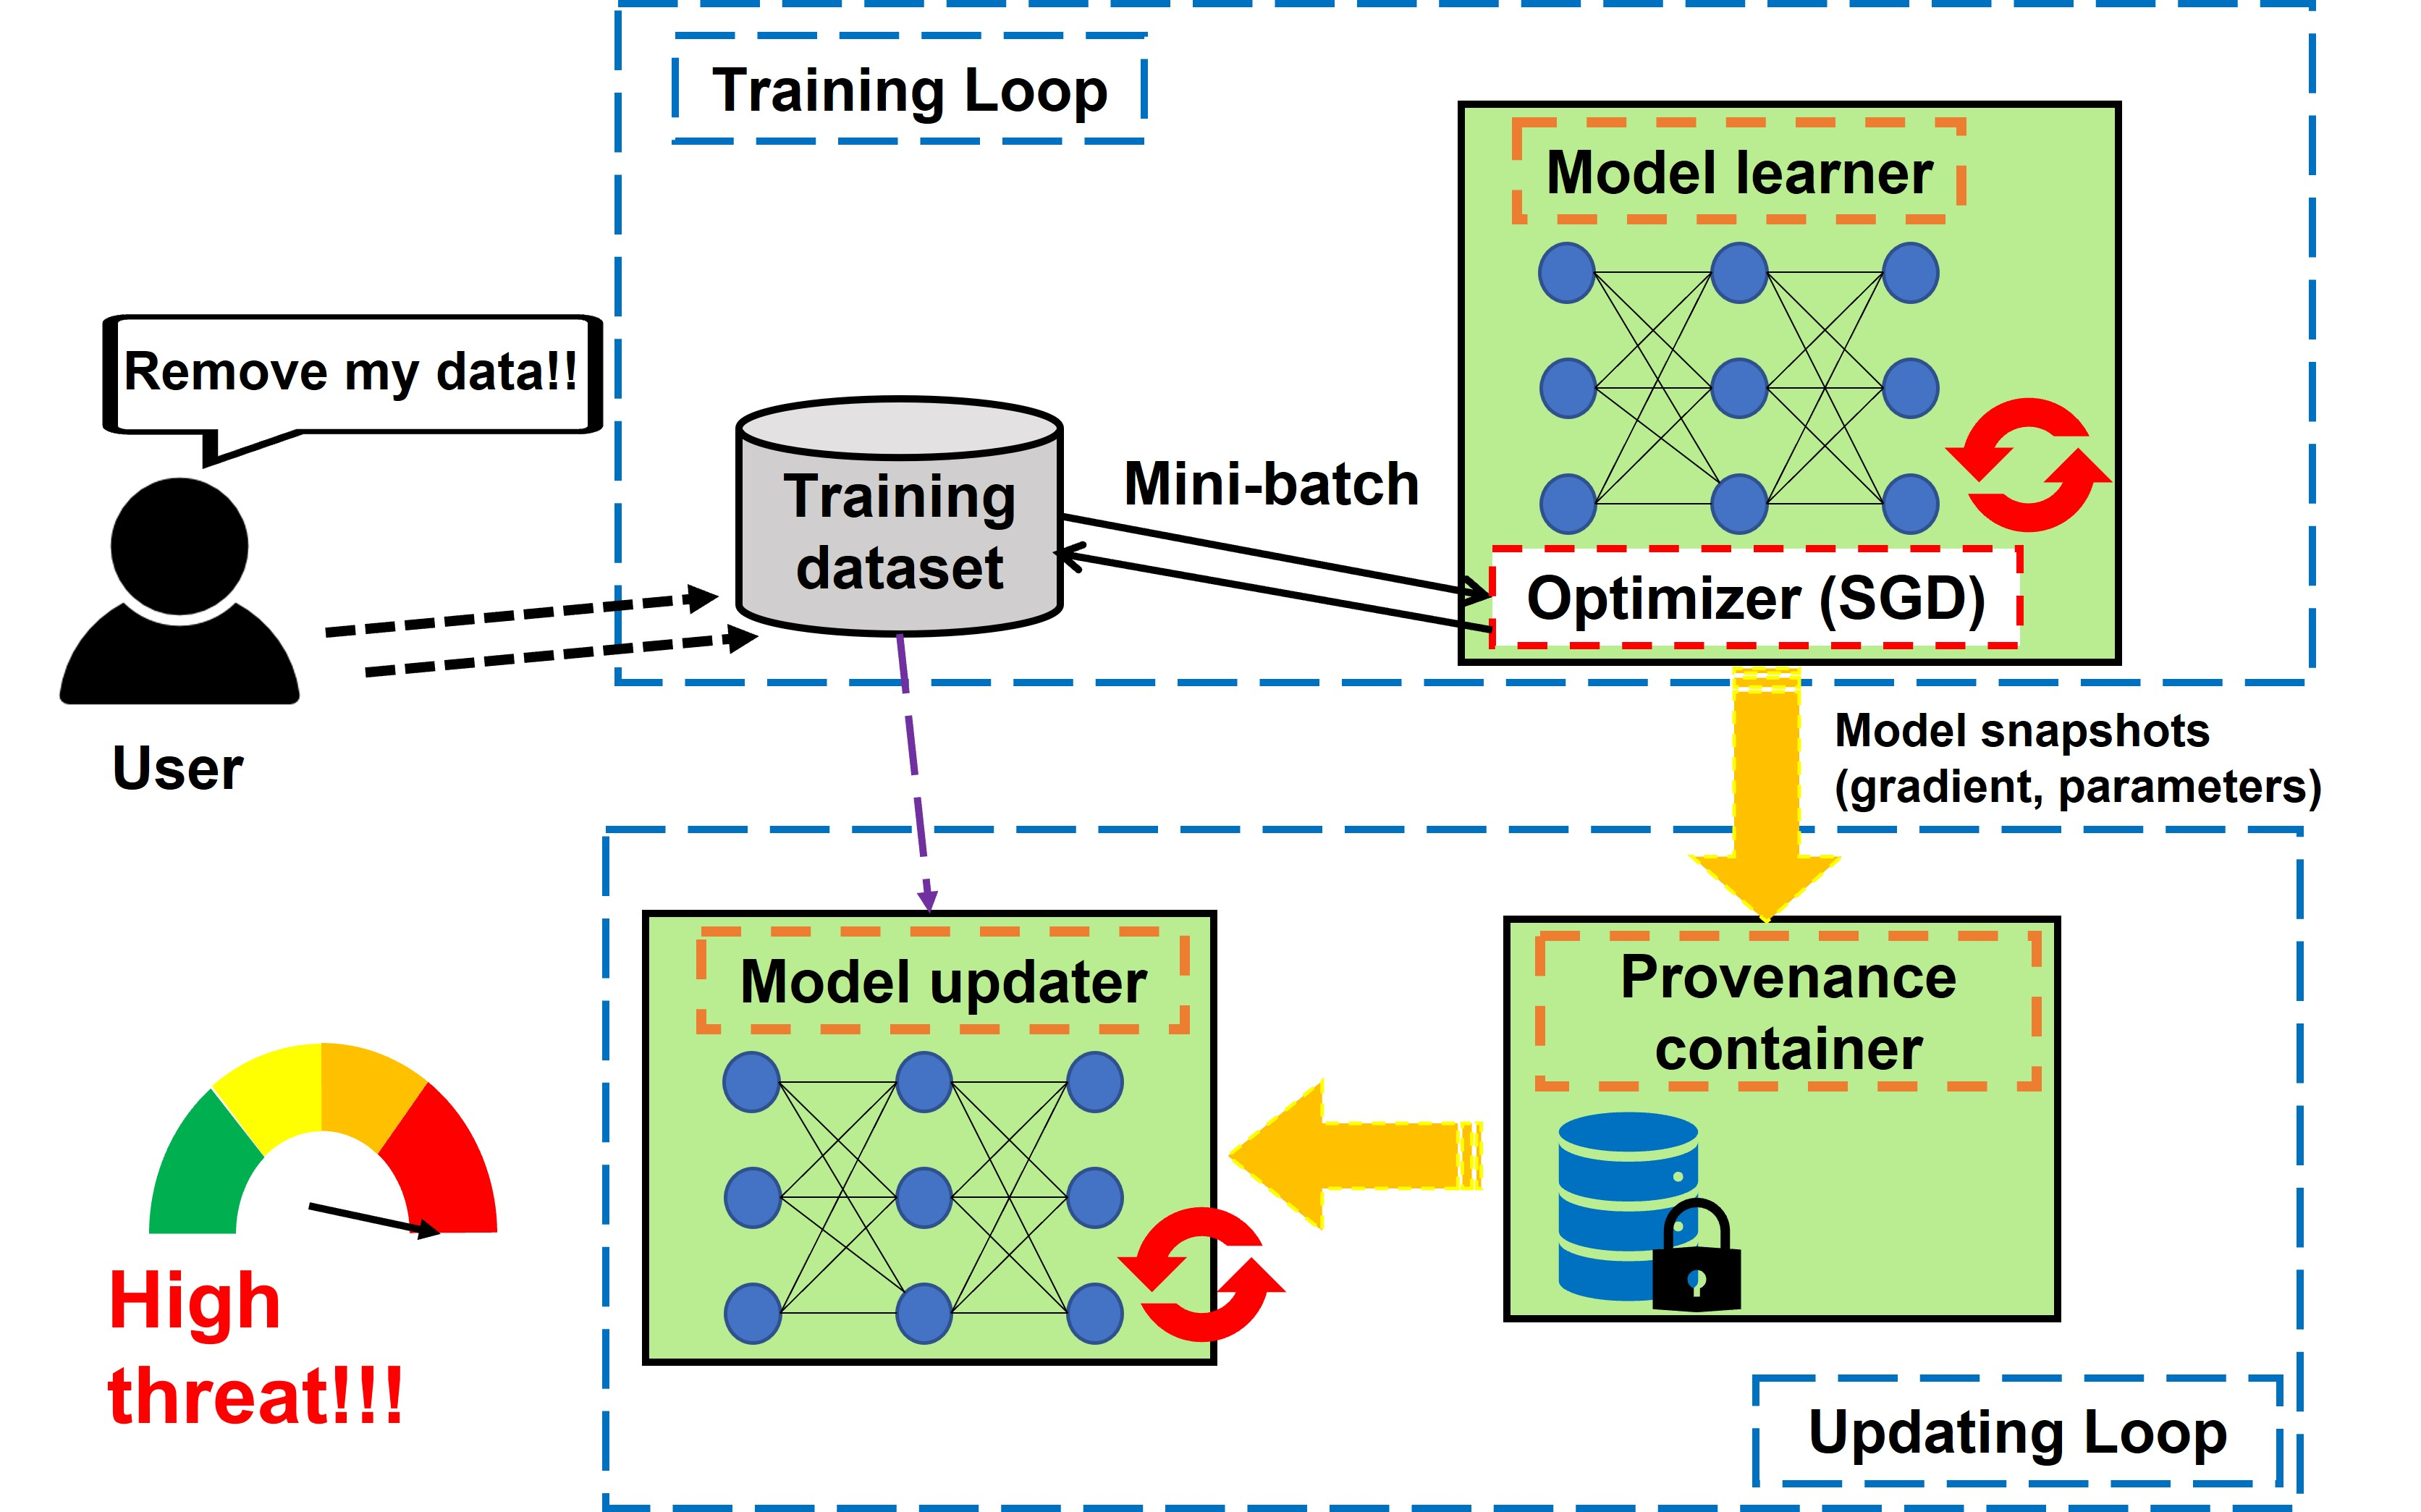
\includegraphics[width=0.65\textwidth, height = 0.4\textwidth, bb=0pt 0pt 700pt 500pt]{figs/pipeline.jpg}
    \caption{Provenance-enabled model unlearning system}
    \label{fig: provenance_enabled_pipeline}
\end{figure}

%talk about the paper making ai forget you

\paragraph*{Challenges and research opportunities} Several challenges remain for developing a provenance-enabled machine unlearning system for general neural network models. First of all, general neural network models are non-convex, which is beyond the model classes that \priu\ or \deltagrad\ support. Therefore, we would envision that a new provenance-based unlearning method is necessary to support incremental updates on general non-convex neural network models. Inspired by \priu\ and \deltagrad, the models incrementally updated in this way could be approximately close to the retrained models, but with rigorous theoretical guarantees on the smallness of the approximation errors. One potential idea to design this new unlearning method is to relax the strong-convexity assumption on the model class in \deltagrad\ such that general non-convex models could be handled. The main bottleneck is the strong dependency of \deltagrad\ on the L-BFGS algorithm, in which the strongly convex objective functions are essential. We notice that this assumption has been relaxed in many extended versions of the L-BFGS algorithm (e.g., \cite{li2001modified}), which could be potentially adapted for extending \deltagrad. 

In addition, due to the high complexity of  state-of-the-art neural neural networks, the model snapshots at each SGD iteration could be extremely large, incurring a prohibitively high overhead for the entire unlearning system. For example, the ResNet18 network for vision tasks has around 11 million parameters \cite{he2016deep} while the GPT-3 model \cite{brown2020language} for natural language processing tasks has around 175 billion parameters. The problem would become even worse if their parameters and gradients were required to be repetitively recorded in the provenance-enabled model unlearning system. As a consequence, it is essential to build a version control system on large neural network models such that the model snapshots could be effectively captured, stored and retrieved. 

One expected characteristic of such a version control system is that the models from different versions (i.e. from different SGD iterations) could be compressed to reduce the storage overhead. Ideally, the compression should be lossless so that the variations between different versions can be captured without adding extra approximation errors after those models are uncompressed during the model update phase. Otherwise, it could potentially amplify the approximation errors brought by the unlearning algorithm itself, thus hurting the quality of the unlearned models. 

The version control problem for machine learning models has been recently studied in~\cite{miao2017towards}. Specifically, the difference between the models from different SGD iterations is calculated first, which can be represented by a set of matrices. Then each element of each matrix, i.e., one float number, is approximately represented with $k$-byte ($k$=16 or 8) integers through the quantization operations. 
This is then followed by compressing the higher-order bits of the quantized representations across different versions of the models throughout the SGD iterations, which can %compress a significant amount of redundant information
yield significant savings (see the experiments of \cite{miao2017towards}). However, since the quantization operations can produce approximation errors, as discussed above, when this solution is applied to the machine unlearning pipeline such errors may lead to significant deviations of the incrementally updated models from the retrained ones.
% the applicability of this solution to the pipeline shown in Figure \ref{fig: provenance_enabled_pipeline} thus depends on whether such errors can 

Another requirement for the provenance-enabled model unlearning system, as shown in Figure \ref{fig: provenance_enabled_pipeline}, is that the collected provenance information be cached in secure storage. Otherwise, the adversary could easily reconstruct the removed training samples from the cached provenance of those samples by using the attack paradigm presented in Section \ref{sec: model_inversion_attack_for_sota}. %This means that it is essential to add a layer in the system to protect the collected provenance data, which may introduce some additional overhead to the entire system.
%
Finally, it is worth noting that the chance of the the security threat mentioned in Section \ref{sec: model_inversion_attack_for_sota} actually occuring may be quite low in practice due to the limited knowledge of the adversary on the models. For instance, in  typical online systems, the deployed machine learning models are released as an open API \footnote{see e.g., Google prediction API: {https://cloud.google.com/ai-platform/prediction/docs/reference/rest/v1/projects/predict}} where the adversary only has black-box access, meaning that only the model output given one input sample can be obtained through the API. In this scenario, it might be inappropriate to use provenance-based unlearning methods due to their relatively high overhead with respect to other unlearning methods. It would be interesting to explore the applicability of existing unlearning methods under different threat assumptions and rank them based on their risk of leaking the removed training samples.


% Note that despite some initial systems on managing the model metadata \cite{vartak2018mistique} in the database community, an efficient version control system for machine learning models still lacks. This, however, can potentially be a critical component for real machine learning model management systems.

% In the worst case, as described in Section \ref{sec: model_inversion_attack_for_sota}, 
% , the model type and the learning algorithm.

% This follows the idea of 

% To our knowledge, despite recent progress on the machine unlearning solutions, the problem of defending against model inversion attacks (thus not violating GDPR) is still not resolved yet. It is still unclear about the applicability of these solutions on defending the ``worst-case'' model inversion attacks. We can imagine that in the worst case, the adversary knows everything about the models, the learning algorithms and even the unlearning algorithms, except the sensitive training samples themselves that are removed by users. In what follows, we aim at demonstrating that to effectively unlearn the models, it is essential to erase the provenance of the removed samples in the training process.

% To illustrate this, suppose 
%the white-box model inversion attack and 
% for a strongly convex model, such as the logistic regression model, one training sample is deleted after the training process on this model
% thus resistant to this attack since it is  
% by assuming that one training sample is deleted and the model is updated afterwards by the \onlinemethod, 

% we can craft the following {\em white-box} attack on the updated model by employing the solution from \cite{guo2020certified}, which aims at incrementally updating linear models (e.g., linear regression and logistic regression models) with L2 regularization. Specifically, suppose the model parameter is $\w_*$ after the training process, then after the removal of the $k_{th}$ training sample, the incrementally updated model parameter is calculated by using a single-step Newton update, i.e.:
% \begin{align*}
    % & \uw_* = \w_* + \bH^{-1}(\w_*; -(\x_k,\y_k))\nabla F(\w_*, (\x_k, \y_k)), \text{where } \bH(\w_*; -(\x_k,\y_k)) = \sum_{i \neq k} \nabla^2 F(\w_*, (\x_i, \y_i))
% \end{align*}



% invoking Equation \eqref{eq: sgd_update0}, i.e. the standard SGD method, on a set of training samples $\{(\x_i, \y_i)\}_{i=1}^n$ for a linear model with parameter $\w^*$ by iteratively invoking 



% 1) undo the \gd\ or \sgd\ updates for $t$ iterations such that the updated models could be rolled back to the model status before the deletions happen, which can be accomplished by performing $t$ iterations of gradient ascent or stochastic gradient ascent on the remaining training samples (recall that $t$ is the number of \gd\ or \sgd\ iterations that the {\em \onlinemethod} requires for incremental updates); 2) estimate the gradient evaluated on the deleted training sample at the current model status by leveraging the fact that the gradient on the full training set is close to zero due to the convergence condition (recall that the adversary may know the remaining training samples after the deletion requests); 3) reconstruct the deleted sample by employing the solution from \cite{zhu2020deep}, which only uses the gradient on the deleted training sample. Note that this problem will not arise for \pro\ and \deltagrad\ as long as the provenance information for incremental updates is not leaked. Intuitively, \pro\ and \deltagrad\ ``erase" the footprint of the deleted training sample from {\em every} \gd\ or \sgd\ iteration so that the gradient evaluated on the removed training sample cannot be obtained by the adversary, thus safeguarding the removed training samples.





%How to defend against the the model inversion attacks in different attack assumptions and different measures of completeness -> propose a general framework that can defend model inversion attacks with provenance-aided model updated approaches






% \input{Sections/challenges}


% \vspace{-.5cm}
\section{Conclusion}
\label{sec:conclusion}

Online job platforms are becoming increasingly popular.
They provide an alternative job arrangement that has the potential to dramatically affect the Future of Work. 
An increasing proportion of human workforce will be employed in such platforms.
Hence, it is very important to study the problem of platform design.
In this paper, we have a preliminary attempt at investigating this problem.
We provide a taxonomy of platforms and what are the major missing functionalities for both workers and requesters. 
We also advocate the need for interoperability between platforms.
This allows workers and requesters to move their data between platforms without getting locked into a single platform. 
There are a number of interesting research and policy challenges in achieving the vision of platform interoperability.

\section{Conclusions}
In this paper, we reviewed our provenance-based techniques, \priu\ and \deltagrad, for incrementally updating machine learning models and showed the connection to incrementally updating database views.  We then studied the privacy implications of machine unlearning techniques, and analyzed the capability of \priu\ and \deltagrad\ as well as other state-of-the-art unlearning techniques on defending against the model inversion attack.  Our analysis reveals that provenance is essential for the unlearning process to guard against this type of attack without hurting performance and the model prediction power. Based on this observation, we envision a provenance-based unlearning system, which could effectively unlearn general machine learning models in a secure manner. We also outlined critical technical challenges and potential solutions, paving the way towards building such systems.

% \noindent
\section*{Acknowledgements}

This material is based upon work that is in part supported by the Defense Advanced Research Projects Agency (DARPA) under Contract No. HR001117C0047.  Partial support was provided by NSF Awards 1547360 and 1733794. Tannen's work at the National University of Singapore was supported in part by the Kwan Im Thong Hood Cho Temple/Avalokite\'{s}vara.

% \eat{
% \begin{thebibliography}{10}  %Must be small, not footnote; contained within the paper; limited to 2 pages.
% \itemsep=1pt
% \begin{small}

% \bibitem{askit2012} R.~Boim, O.~Greenshpan, T.~Milo, S.~Novgorodov, N.~Polyzotis, and W.-C. Tan. \newblock Asking the right questions in crowd data sourcing. \newblock {\em ICDE}, 0:1261–1264, 2012.

% \end{small}
% \end{thebibliography}
% }
% \susan{using this bib style for now, must change for final version to include in the document itself}
% \bibliographystyle{alpha}
% \bibliography{refs}

\begin{thebibliography}{10}
\itemsep=1pt
\begin{small}

\bibitem{voigt2017eu} P.~Voigt, and A. Von dem Bussche
% R.~Boim, O.~Greenshpan, T.~Milo, S.~Novgorodov, N.~Polyzotis, and W.-C. Tan. 
\newblock The eu general data protection regulation (gdpr). \newblock {\em A Practical Guide, 1st Ed., Cham: Springer International Publishing}, 2017.

\bibitem{quenouille1956notes} M. H. Quenouille, 
% R.~Boim, O.~Greenshpan, T.~Milo, S.~Novgorodov, N.~Polyzotis, and W.-C. Tan. 
\newblock Notes on bias in estimation. \newblock {\em Biometrika}, 43 (3/4), pp.353-360, 1956.

\bibitem{politis1999subsampling} D. N. Politis, and J. P. Romano and M. Wolf 
\newblock Subsampling. \newblock {\em Springer Science \& Business Media}, 1999.

\bibitem{ghorbani2019data} A. Ghorbani, and J. Zou. \newblock Data shapley: Equitable valuation of data for machine learning. \newblock{\em  In International Conference on Machine Learning}, pp. 2242-2251. PMLR, 2019.

\bibitem{DBLP:journals/debu/GuptaM95} A.~Gupta, and I.~S.~Mumick. \newblock Maintenance of materialized views: Problems, techniques, and applications. \newblock{\em IEEE Data Eng. Bull.}, 18(2), pp.3-18., 1995

\bibitem{lab2009} A.~Labrinidis, and Y.~Sismanis. \newblock View Maintenance, pages 3326–3328. \newblock{\em Springer}, Boston, MA, 2009.


\bibitem{GreenKT07} T.~J.~Green, G.~Karvounarakis, and V.~Tannen,  \newblock Provenance semirings. \newblock{\em In Proceedings of the twenty-sixth ACM SIGMOD-SIGACT-SIGART symposium on Principles of database systems} pp. 31-40, 2007.

\bibitem{yan2016fine} Z.~Yan, V.~Tannen, and Z.~G.~Ives. \newblock Fine-grained Provenance for Linear Algebra Operators. In \newblock{\em TaPP}. 2016.

\bibitem{wu2020priu} Y.~Wu, V.~Tannen, and S.~B.~Davidson. \newblock Priu: A provenance-based approach for incrementally updating regression models. \newblock{\em In Proceedings of the 2020 ACM SIGMOD International Conference on Management of Data}, pp. 447-462. 2020.

\bibitem{wu2020deltagrad} Y.~Wu, E.~Dobriban, and S.~B.~Davidson. \newblock DeltaGrad: Rapid retraining of machine learning models. \newblock{\em In International Conference on Machine Learning}, pp. 10355-10366. PMLR, 2020.

\bibitem{bourtoule2021machine} L.~Bourtoule, V.~Chandrasekaran, C.~A.~Choquette-Choo, H.~Jia, A.~Travers, B.~Zhang, D.~Lie, and N.~Papernot. \newblock Machine unlearning. \newblock {\em In 2021 IEEE Symposium on Security and Privacy (SP)}, pp. 141-159, 2021.

\bibitem{fredrikson2015model} M.~Fredrikson, S.~Jha, and T.~Ristenpart. \newblock Model inversion attacks that exploit confidence information and basic countermeasures. \newblock {\em In Proceedings of the 22nd ACM SIGSAC conference on computer and communications security}, pp. 1322-1333. 2015.

\bibitem{amsterdamer2011provenance} Y.~Amsterdamer, D.~Deutch, and V.~Tannen. \newblock Provenance for aggregate queries. \newblock{\em In Proceedings of the thirtieth ACM SIGMOD-SIGACT-SIGART symposium on Principles of database systems}, pp. 153-164. 2011.

\bibitem{mokhtari2015global} A.~Mokhtari, and A.~Ribeiro. \newblock Global convergence of online limited memory BFGS. \newblock{\em The Journal of Machine Learning Research} 16, no. 1 (2015): 3151-3181.

\bibitem{guo2020certified} C.~Guo, T.~Goldstein, A.~Hannun, and L.~Van Der Maaten.\newblock Certified Data Removal from Machine Learning Models. \newblock{\em In International Conference on Machine Learning}, pp. 3832-3842. PMLR, 2020.


\bibitem{neel2021descent} S.~Neel, A.~Roth, and S.~Sharifi-Malvajerdi. \newblock Descent-to-delete: Gradient-based methods for machine unlearning. \newblock{\em In Algorithmic Learning Theory}, pp. 931-962. PMLR, 2021.

\bibitem{dwork2014algorithmic} C.~Dwork, and A.~Roth. \newblock The algorithmic foundations of differential privacy. \newblock{\em Found. Trends Theor. Comput. Sci.} 9, no. 3-4 (2014): 211-407.

\bibitem{izzo2021approximate} Z.~Izzo, M.~A.~Smart, K.~Chaudhuri, and J.~Zou. \newblock Approximate data deletion from machine learning models. \newblock{\em In International Conference on Artificial Intelligence and Statistics}, pp. 2008-2016. PMLR, 2021.

\bibitem{zanella2020analyzing} S.~Zanella-Béguelin, L.~Wutschitz, S.~Tople, V.~Rühle, A.~Paverd, O.~Ohrimenko, B.~Köpf, and M.~Brockschmidt. \newblock Analyzing information leakage of updates to natural language models. \newblock{\em In Proceedings of the 2020 ACM SIGSAC Conference on Computer and Communications Security}, pp. 363-375. 2020.

\bibitem{golatkar2020forgetting} A.~Golatkar, A.~Achille, and S.~Soatto. \newblock Forgetting outside the box: Scrubbing deep networks of information accessible from input-output observations. \newblock{\em In European Conference on Computer Vision}, pp. 383-398. Springer, Cham, 2020.

\bibitem{koh2017understanding} P.~W.~Koh, and P.~Liang. \newblock Understanding black-box predictions via influence functions. \newblock{\em In International Conference on Machine Learning}, pp. 1885-1894. PMLR, 2017.

\bibitem{martens2010deep} J.~Martens.\newblock Deep learning via hessian-free optimization. In \newblock{\em ICML}, vol. 27, pp. 735-742. 2010.


\bibitem{agarwal2016second} N.~Agarwal, B.~Bullins, and E.~Hazan. \newblock Second-order stochastic optimization in linear time. \newblock{\em stat} 1050 (2016): 15.

\bibitem{sherman1950adjustment} J.~Sherman, and W.~J.~Morrison. \newblock Adjustment of an inverse matrix corresponding to a change in one element of a given matrix. \newblock{\em The Annals of Mathematical Statistics} 21, no. 1 (1950): 124-127.

\bibitem{kraska2018case} T.~Kraska, A.~Beutel, E.~H.~Chi, J.~Dean, and N.~Polyzotis. \newblock The case for learned index structures. \newblock{\em In Proceedings of the 2018 International Conference on Management of Data}, pp. 489-504. 2018.


\bibitem{marcus12neo} R.~Marcus, P.~Negi, H.~Mao, C.~Zhang, M.~Alizadeh, T.~Kraska, O.~Papaemmanouil, and N.~Tatbul. \newblock Neo: A Learned Query Optimizer. \newblock{\em Proceedings of the VLDB Endowment} 12, no. 11.

\bibitem{shu2019meta} J.~Shu, Q.~Xie, L.~Yi, Q.~Zhao, S.~Zhou, Z.~Xu, and D.~Meng. \newblock Meta-Weight-Net: Learning an Explicit Mapping For Sample Weighting. \newblock {\em Advances in Neural Information Processing Systems} 32 (2019): 1919-1930.

\bibitem{ginart2019making} A.~Ginart, M.~Guan, G.~Valiant, and J.~Zou. \newblock Making AI Forget You: Data Deletion in Machine Learning. \newblock{\em Advances in neural information processing systems} (2019).

\bibitem{li2001modified} D.~Li, and M.~Fukushima. \newblock A modified BFGS method and its global convergence in nonconvex minimization. \newblock{\em Journal of Computational and Applied Mathematics} 129, no. 1-2 (2001): 15-35.

\bibitem{he2016deep} K.~He, X.~Zhang, S.~Ren, and J.~Sun. \newblock Deep residual learning for image recognition. \newblock{\em In Proceedings of the IEEE conference on computer vision and pattern recognition}, pp. 770-778. 2016.

\bibitem{brown2020language} T.~B.~Brown, B.~Mann, N.~Ryder, M.~Subbiah, J.~Kaplan, P.~Dhariwal, A.~Neelakantan et al. \newblock Language Models are Few-Shot Learners. \newblock{\em arXiv e-prints (2020)}: arXiv-2005.

\bibitem{miao2017towards} H.~Miao, A.~Li, L.~S.~Davis, and A.~Deshpande. \newblock Towards unified data and lifecycle management for deep learning. \newblock{\em In 2017 IEEE 33rd International Conference on Data Engineering (ICDE)}, pp. 571-582. IEEE, 2017.

\end{small}
\end{thebibliography}











\end{document}
